\documentclass[preprint,russian,a5paper,10pt,twoside,mediummath]{ncc}
\usepackage[utf8]{inputenc}
\usepackage{misccorr}			% различные особенности оформления документов, принятые в России
\usepackage{indentfirst}		% начинать абзац с красной строки
\usepackage{tikz}				% рисование чертежей
\usetikzlibrary{positioning}	% автоматическое размещение элементов на чертежах относительно друг друга
\usetikzlibrary{shapes.misc}
\usepackage{enumitem}			% Для разрывов в списках
\usepackage{ncccomma}			% для использования запятой в качестве разделителя дробной части
\usepackage{framed}				% текст в рамке

\pagestyle{plain}
\countstyle{section}			% посекционная нумерация

%********Команда все примеры подчеркиваем
\newcommand{\ExampleMy}{\vspace{\baselineskip}\textbf{\underline{Пример:}}\nopagebreak\par}
%*********

\newcounter{problem}[section]				% счётчик примеров (имя example уже зарезервировано)
\renewcommand{\theproblem}{\thesection.\arabic{problem}}		% команда вывода текущего значения счётчика примеров
% окружение для оформления примера
\newenvironment{problem}{\par\refstepcounter{problem}{\raggedleft\textit{Пример \theproblem}\par}\begin{oframed}}{\par\end{oframed}}

\begin{document}

\begin{titlepage}
	\titlehead{\footnotesize САНКТ-ПЕТЕРБУРГСКИЙ\\ ГОСУДАРСТВЕННЫЙ ПОЛИТЕХНИЧЕСКИЙ УНИВЕРСИТЕТ\par\vspace{1mm} ИНСТИТУТ ИНФОРМАЦИОННЫХ ТЕХНОЛОГИЙ И УПРАВЛЕНИЯ\par\vspace{1mm} КАФЕДРА КОМПЬЮТЕРНЫХ СИСТЕМ\\ И ПРОГРАММНЫХ ТЕХНОЛОГИЙ}
	\titlefoot{Санкт-Петербург\\ \theyear}
	\author{С.\=,А.~Нестеров}
	\title{СИСТЕМЫ ОПТИМАЛЬНОГО УПРАВЛЕНИЯ}
	\titlecomment{Конспект лекций}
	\maketitle
\end{titlepage}

\setcounter{page}{2}
\thispagestyle{empty}
\mbox{}\newpage
\tableofcontents
\newpage

\setcounter{secnumdepth}{-1}		% отключили нумерацию разделов
\section{Введение\label{intro}}
\setcounter{secnumdepth}{2}		% включили обратно

Для начала определимся, что понимается под управлением. Существует три фундаментальных принципа управления:
\begin{itemize}
\item Управление по заданию --- необходимо получить заданный сигнал $v$ на выходе объекта управления (ОУ). Для этого передаточная функция системы управления в целом (см. рис.~\ref{fig:intro:control_by_target}) должна быть равна единице. Тогда передаточная функция уст\-ройства управления (УУ) равна:
\begin{equation}\label{equ:intro:control_by_target}
W_{\text{\textit{УУ}}}=\frac{1}{W_{\text{\textit{ОУ}}}}
\end{equation}

\begin{figure}[ht] \centering		% [ht] - размещение в указанном месте, а если невозможно, то вверху следующей страницы
\begin{tikzpicture}											% здесь размеры по умолчанию в см
	[	auto,												% чтобы элементы чертежа не пересекались
		inner sep = 2ex,									% пространство, оставляемое вокруг текста
		block/.style={rectangle,draw=black,thick},		% стиль отрисовки блока
		vec/.style={->,>=stealth,semithick},				% стиль отрисовки вектора
		point/.style={inner sep = 0pt}	]
	\node[block] (object) {$ W_{\text{\textit{ОУ}}} $};	% Ставить ; обязательно! ИНАЧЕ ВСЁ ВИСНЕТ!!!!1
	\node[block] (regulator) [left = of object] {$ W_{\text{\textit{УУ}}} $};
%	\draw[vec] (regulator) to (object);					% вектор без подписи
	\draw[vec] (regulator) to node{$u$} (object);			% вектор с подписью
	\node[point] (input) [left = of regulator] {};
	\draw[vec] (input) to node{$v$} (regulator);
	\node[point] (output) [right = of object] {};
	\draw[vec] (object) to node{$x$} (output);
\end{tikzpicture}
\footnotesize \caption{Управление по заданию\label{fig:intro:control_by_target}}
\end{figure}

\item Управление по возмущению --- возмущения $f$, действующие на объект, учитываются при формировании управляющего воздействия $u$ (см. рис.~\ref{fig:intro:control_by_noise}). Передаточная функция от возмущений к выходу может быть выражена как $ W_{fu}W_\text{\textit{ОУ}}+W_{fx} $ и должна быть равна нулю. Тогда передаточная функция от возмущений к управлению равна:
\begin{equation}\label{equ:intro:control_by_noise}
W_{fu}=-\frac{W_{fx}}{W_\text{\textit{ОУ}}}
\end{equation}

\begin{figure}[ht] \centering
\begin{tikzpicture}	
	[	auto, inner sep = 2ex,
		block/.style={rectangle,draw=black,thick},
		vec/.style={->,>=stealth,semithick},
		point/.style={inner sep = 0pt}	]
	\node[block] (object) {$ W_\text{\textit{ОУ}} $};
	\node[block] (regulator) [left = of object] {$ W_\text{\textit{УУ}} $};
	\draw[vec] (regulator) to node{$u$} (object);
	\node[point] (input) [left = of regulator] {};
	\draw[vec] (input) to node{$v$} (regulator);
	\node[point] (output) [right = of object] {};
	\draw[vec] (object) to node{$x$} (output);
	\node[point] (noise) [above = of object] {};
	\draw[vec] (noise) to node(f){$f$} (object);
	\draw[vec] (f.west) -| (regulator.north);
	\fill (f.west) circle (1pt);
\end{tikzpicture}
\footnotesize \caption{Управление по возмущению\label{fig:intro:control_by_noise}}
\end{figure}

\item Управление по ошибке --- на вход регулятора подаётся отклонение $e$ выходного сигнала объекта $x$ от сигнала задания $v$ (см. рис.~\ref{fig:intro:control_by_eps}). Если $e$ устремить к нулю, то передаточная функция от $e$ к $x$ должна устремиться к бесконечности, чтобы получить на выходе заданную величину:
\begin{equation}\label{equ:intro:control_by_eps}
W_\text{\textit{УУ}}W_\text{\textit{ОУ}}\longrightarrow\frac{x_\text{\textit{уст}}}{0}=\infty
\end{equation}

Этого можно добиться, например, введением в регулятор очень больших коэффициентов усиления или интегрирующих звеньев.

\begin{figure}[ht] \centering
\begin{tikzpicture}	
	[	auto, inner sep = 2ex,
		block/.style={rectangle,draw,thick},
		vec/.style={->,>=stealth,semithick},
		point/.style={inner sep = 0pt}	]
	\node[block] (object) {$ W_\text{\textit{ОУ}} $};
	\node[block] (regulator) [left = of object] {$ W_\text{\textit{УУ}} $};
	\draw[vec] (regulator) to node{$u$} (object);
	\node[circle,draw,thick,inner sep=0pt,minimum size=2ex] (sum) [left = of regulator] {};
	\draw[semithick] (sum.north west) -- (sum.south east);
	\draw[semithick] (sum.south west) -- (sum.north east);
	\fill (sum.center) -- (sum.south west) arc (-135:-45:1ex) -- cycle;
	\draw[vec] (sum) to node{$e$} (regulator);
	\node[point] (input) [left = of sum] {};
	\draw[vec] (input) to node{$v$} (sum);
	\node[point] (output) [right = of object] {};
	\draw[vec] (object) to node(x){$x$} (output);
	\node[point] (p1) [below=of sum] {};
	\draw (x.south) |- (p1.center) [vec] to (sum);
	\fill (x.south) circle (1pt);
\end{tikzpicture}
\footnotesize \caption{Управление по ошибке\label{fig:intro:control_by_eps}}
\end{figure}
\end{itemize}
% Смотри формулу~\eqref{equ:intro:control_by_target}, с.~\pageref{equ:intro:control_by_target}.
% А теперь смотри рисунок~\ref{fig:intro:control_by_target}, с.~\pageref{fig:intro:control_by_target}.

По решаемой задаче системы автоматического управления (САУ) можно разделить на системы:
\begin{itemize}
\item стабилизации
\item программного управления
\item слежения
\item оптимального управления
\item адаптивного управления (поисковые и самонастраивающиеся)
\end{itemize}

Анализ и синтез САУ предполагает, что кроме цели рассматривается путь решения задачи. Для этого используются различные показатели качества:
\begin{itemize}
\item Прямые:
	\begin{itemize}
	\item Статические: статизм, добротность;
	\item Динамические: время переходного процесса, перерегулирование, колебательность;
	\end{itemize}
\pagebreak
\item Косвенные:
	\begin{itemize}
	\item Корневые;
	\item Частотные;
	\item Интегральные.
	\end{itemize}
\end{itemize}

Существует два основных подхода к синтезу САУ:
\begin{enumerate}
\item Обеспечить заданные показатели качества;
\item Обеспечить наилучшее (оптимальное) в каком-либо определённом смысле качество управления для заданного объекта при конкретных условиях работы и ограничениях.
\end{enumerate}

Эти два подхода имеют право на жизнь и естественно широко применяются. При этом надо понимать, что второй подход даёт максимально возможный (в отличие от первого, который даёт минимально пригодный) результат. Однако, за предельно достижимое качество необходимо будет чем-то \glqq заплатить\grqq. Поэтому должно быть оценено, что даёт выигрыш в качестве и чем за это надо \glqq заплатить\grqq. Соответственно, дальнейшее и посвящено рассмотрению теоретических моментов по расчёту и реализации соответствующих систем.

При решении такой задачи естественно требовать от управляемого процесса (ОУ) выполнения условий полной управляемости и наблюдаемости.

\clearpage		% выводит все накопившиеся плавающие элементы, а затем завершает страницу

\section{Постановка задачи оптимального управления\label{task}}

В общем случае постановки задач оптимального управления характеризуются значительным разнообразием, что связано с тремя основными причинами:
\begin{itemize}
\item Конкретными \glqq условиями\grqq функционирования, к которым следует отнести:
\begin{itemize}
\item начальное (исходное) и конечное (требуемое) состояния ОУ с временной привязкой $X_{0}\left ( t_{0} \right )$, $X_\text{\textit{к}}\left ( t_\text{\textit{к}} \right )$;
\item взаимосвязи, присущие реальным процессам, в форме:
\begin{itemize}
\item алгебраических (голономных) уравнений $G\left(x,u\right)=0$,
\item дифференциальных (неголономных) уравнений\\ $\varphi \left( x,u,t \right)=\dot{x}-Ax+Bu=0$,
\item интегральных (изопериметрических) уравнений\\ $I\left( x,u,t \right)=\int\limits_{t_0}^{t_\text{\textit{к}}}{\varphi \left( x,u,t \right)dt=C}$;
\end{itemize}
\end{itemize}
\item Ограничениями на управляющие сигналы и переменные состояния $\underline{U}\le U\le \overline{U}$; $\underline{X}\le X\le \overline{X}$; $\sum\limits_{i=1}^{n}{u_{i}^{2}}\le A$
\item Математическим видом критерия оптимальности.
\end{itemize}

Выбор критерия не является формальным актом, он не предписывается какой-либо теорией, а полностью определяется содержанием задачи управления. В общем виде критерий записывается функционалом:
\begin{equation}\label{equ:task:criterion_general}
J \left( U, X, \underset{t_\text{\textit{к}} - t_0}{\mathop{T}} \, \right) = \Phi \left( \underset{X_0, \, X_\text{\textit{к}}}{\mathop{ X \left( T \right) }} , T \right) + \int\limits_{t_0}^{t_\text{\textit{к}}} F\bigl( X(t), U(t), t \bigr) \, dt,
\end{equation}
где $ \Phi \bigl( X(T), T \bigr) $ --- терминальная составляющая, характеризующая качество управления только по начальному и конечному состояниям ОУ (поэтому отсутствует $U$); $ F \bigl( X(t), U(t), t \bigr) $ --- подынтегральная целевая функция, характеризующая качество внутри интервала управления. Управление должно обеспечивать экстремальное значение критерия оптимальности $ U = \underset{U}{\mathop{extr}} \, J \left( X, U, T \right) $. \smallskip 

Вид критерия $ J( X, U, T) $ задаёт класс задач оптимальности:
\begin{enumerate}
\item Критерий максимального быстродействия (минимального времени реакции):
\begin{enumerate}
\item[а)] $ \Phi \bigl( X(T), T \bigr) = T = t_\text{\textit{к}} - t_0 , \quad F\bigl( X(t), U(t), t \bigr) \equiv 0 $  
\item[б)] $ \Phi \bigl( X(T), T \bigr) \equiv 0 , \quad F\bigl( X(t), U(t), t \bigr) = 1 \to \int\limits_0^T 1\,dt = T $
\end{enumerate}

%\begin{subequations}\label{equ:task:minT}
%\renewcommand{\theequation}{\theparentequation\asbuk{equation}}
%\begin{equation}\label{equ:task:minT_first}
%y = x
%\end{equation}
%\begin{equation}\label{equ:task:minT_second}
%z = x^2(C+1)
%\end{equation}
%\end{subequations}

\item Критерий минимального расхода управления (топлива):
\[ \Phi \bigl( X(T), T \bigr) \equiv 0 , \quad F \bigl( X(t), U(t), t \bigr) = R \left| U \right| = \sum\limits_{i=1}^{n}{ r_i \left| u_i \right| } \]
\item Критерий предельной точности (минимальной ошибки):
\[ \Phi \bigl( X(T), T \bigr) \equiv 0, \quad F \bigl( X(t), U(t), t \bigr) = X^TQX, \] где $X$ --- отклонение (ошибка) от заданного значения, $Q$ --- матрица весовых коэффициентов (важность каждой составляющей в общей ошибке).
\item Критерий минимума энергетических затрат:
\[ \Phi \bigl( X(T), T \bigr) \equiv 0, \quad F \bigl( X(t), U(t), t \bigr) = U^TRU = \sum\limits_{i=1}^{n}{r_i u_i^2} \] на интервале $ t_\text{\textit{к}} - t_0 = T $
\item Критерий терминального управления (задача мягкой посадки или система управления конечным положением):
\[ \Phi \bigl( X(T), T \bigr) \ne 0, \quad F \bigl( X(t), U(t), t \bigr) \equiv 0 \]
\end{enumerate}
\pagebreak
Часто используются смешанные варианты критериев:
\begin{enumerate}[resume]
\item Квадратичный критерий качества управления (предельной точности при минимуме энергетических затрат):
\[ \Phi \bigl( X(T), T \bigr) \equiv 0, \quad F \bigl( X(t), U(t), t \bigr) = X^TQX + U^TRU \]
\item Критерий максимального быстродействия при минимальном расходе топлива (для управления автономными ОУ):
\[ \Phi \bigl( X(T), T \bigr) \equiv 0, \quad F \bigl( X(t), U(t), t \bigr) = 1 + R\left|U\right| = 1 + \sum\limits_{i=1}^{n}{ r_i \left| u_i \right| } \]
\item Критерий минимизации энергетических затрат при фиксированном интервале времени и заданном состоянии: 
\[ J = X^T \left( T \right) S X \left( T \right) + \int\limits_0^T \left( X^TQX + U^TRU \right) \, dt \] 
\end{enumerate}

Постановки задачи с критерием общего вида (двумя слагаемыми) принято называть задачей в форме Больца; терминальные постановки (только первое слагаемое) --- в форме Майера; постановки только с интегралом (без первого слагаемого) --- в форме Лагранжа.

%Вывод первого раздела
В итоге: задачи оптимального управления являются задачами минимизации на множестве функций и могут быть решены методами классического вариационного исчисления. Однако, наличие ограничений в форме равенств (уравнения УП и ОУ) и особенно в форме неравенств (ограничения допустимых управлений и состояний) требует применения методов неклассического вариационного исчисления, к которым относятся принцип максимума Л.\=,С.~Понтрягина, метод динамического программирования Р.~Беллмана, метод моментов Н.\=,Н.~Красовского, симплекс-метод линейного программирования, метод нелинейного программирования Табака-Куо, Куна-Таккера, символьные методы решения нелинейных алгебраических (например, трансцендентных) уравнений и~т.\,п. (градиентные и методы прямого поиска).


%Часть 3 Теория решения задач на экстремум
\clearpage
\section{Теория решения задач на экстремум\label{extremum}}
Формально достаточно общие задачи на отыскание $\max$  или $\min$ функции записываются в виде $\underset{x}{\mathop{extr}} \, F \left( x \right) $, $ x \in X $, т.\=,е.~найти в множестве $X$ точку $x$, при которой скалярная функция векторного аргумента $F \left( x \right) $ принимает экстремальное значение. При этом точки $ x = {\left( x_1, x_2, \dots x_n \right)}^T \in X$ называют допустимыми, само множество может быть ограничено или $ X \in \mathop{R}^n $, а задача поиска $ \max \, F\left( x \right) $ сведена к задаче поиска $ \min \, { - F \left( x \right) }$. Точку $ x^* \in \mathop{X}^* $ такую, что $ F \left( x^* \right) \underset{\le}{\ge} F \left( x \in X, \, x \ne x^* \right) $ называют решением задачи на $ \underset{\min}{\max} $ (экстремум), а $ F \left( x^* \right) $ --- значением экстремума.

Для сложных функций в заданной области может быть несколько таких точек (локальные экстремумы, также называемые слабыми, и абсолютные экстремумы, также называемые сильными).

Для отыскания решения задачи без ограничений необходимо:
\begin{itemize}
\item выписать условия экстремума:
\begin{equation}\label{equ:extremum:general}
grad \, F \left( x \right) = \frac{\partial F\left( x \right)}{\partial x} = 0
\end{equation}
(для скалярного аргумента: $\frac{df}{dx}=0$ );
\item найти решения этих уравнений --- полученные решения называют стационарными точками;
\item отыскать среди них решения задачи или доказать, что его нет. Достаточным условием решения задачи на $\max$ ($\min$) является отрицательная (положительная) определённость матрицы вторых производных $ \frac{ \partial ^ 2 F \left( x \right) }{ \partial x ^ 2} $ --- матрицы Гессе.
\end{itemize}

%**********
%Надо как-то выделить текст
%**********
%Пример
%\par\ExampleMy 
\begin{problem}
$ \min \, F \left( x \right) = \frac{1}{2} \left( x_1^2 + 4x_2^2 \right) $
\[ \left\{ \begin{darray}{l}
   \frac{\partial F}{\partial x_1} = x_1 \nr
   \frac{\partial F}{\partial x_2} = 4x_2
\end{darray} \right. \equiv 0 \enskip \Rightarrow \enskip \left\{ \begin{darray}{l}
   x_1 = 0 \\
   x_2 = 0
\end{darray} \right. \enskip \Rightarrow \enskip
\frac{ \partial ^ 2 F }{ \partial x ^ 2} = \left| \begin{matrix} 1 & 0 \\ 0 & 4 \end{matrix} \right| \]
Положительная определённость может быть подтверждена вычислением собственных чисел ($ \lambda _ 1 = 1, \lambda _ 2 = 4 $) или анализом всех диагональных миноров ($ \Delta _ 1 = 1, \Delta _2 = 4 $). Это доказывает, что стационарная точка $ \left( 0, 0 \right) $ абсолютный (глобальный) $\min$.
\end{problem}
\begin{problem}
$ \min \, F \left( x \right) = x_1^2 - 2 x_1 x_2 + 4 x_2^2 $
\[ \left\{ \begin{darray}{l}
   \frac{\partial F}{\partial x_1} = 2 x_1 - 2 x_2 = 0  \nr
   \frac{\partial F}{\partial x_2} = -2 x_1 + 8 x_2 = 0
\end{darray} \right. \enskip \Rightarrow \enskip x^* = {\left( 0, 0 \right)}^T \]
Матрица Гессе $ \frac{ \partial ^ 2 F }{ \partial x^2 } =
\left| \begin{array}{@{}rr@{}} 	% выравнивание обоих столбцов по правому краю
	 2 & -2 \\
	-2 &  8
\end{array} \right| $ положительно определённая --- это достаточное условие $ \min \, F \left( x^* \right) = 0 $
\end{problem}
\begin{problem}
$ f(x) = x^3 \left( x^2 - 1 \right) \to extr; \quad -1 \le x \le 2 $
\[ \frac{\partial f}{\partial x} = 5x^4 - 3x^2 = 0 \enskip \Rightarrow \enskip x_1 = 0, x_2 = \sqrt{3/5}, x_3 = - \sqrt{3/5} \]
\[ \frac{\partial ^ 2 F }{\partial x^2} = 20x^2 - 6x \]
\[ \left\{ \begin{darray}{l}
	\frac{\partial ^ 2 F }{\partial x^2} \Big| _{x=x_1} = 0 \nr
	\frac{\partial ^ 2 F }{\partial x^2} \Big| _{x=x_2} = 6\sqrt{3/5} > 0 \enskip \Rightarrow \min \nr
	\frac{\partial ^ 2 F }{\partial x^2} \Big| _{x=x_3} = -6\sqrt{3/5} < 0 \enskip \Rightarrow \max
\end{darray} \right. \]
\[ f \left( x_1 \right) = 0; \enskip f \left( x_2 \right) = - \frac{6}{25} \sqrt{\frac{3}{5}} \approx - 0,2; \enskip f \left( x_3 \right) = \frac{6}{25} \sqrt{\frac{3}{5}} \approx 0,2\]
\[ f(-1) = 0; \enskip f(2) = 24 \]
\end{problem}

\begin{figure}[ht] \centering
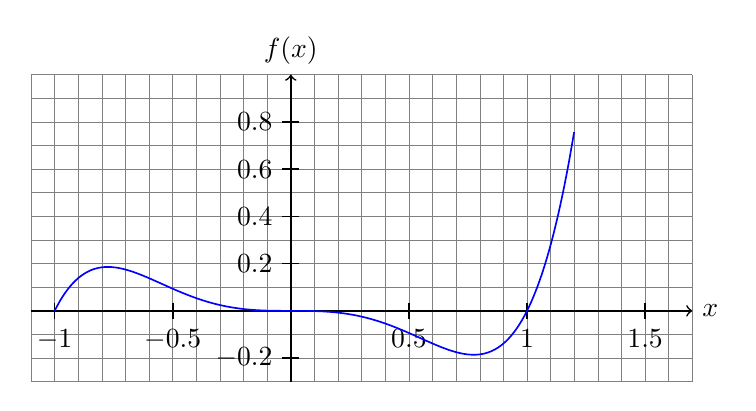
\begin{tikzpicture}
	[	scale=3,				% масштаб (относительно 1см)
		smooth,					% сглаживать углы
		samples=100,			% число точек на графике
		domain=-1:1.2	]		% диапазон значений входной величины
	\draw[very thin,gray,step=1 mm] (-1.1,-0.3) grid (1.7,1);		% сетка
	\draw[semithick,->] (-1.1,0) -- (1.7,0) node[right] {$x$};			% ось абсцисс
	\draw[semithick,->] (0,-0.3) -- (0,1) node[above] {$f(x)$};		% ось ординат
	\foreach \x in {-1,-0.5,0.5,1,1.5}
		\draw[semithick] (\x cm,1pt) -- (\x cm,-1pt) node[anchor=north] {$\x$};
	\foreach \y in {-0.2,0.2,0.4,0.6,0.8}
		\draw[semithick] (1pt,\y cm) -- (-1pt,\y cm) node[anchor=east] {$\y$};
	\draw[semithick,blue] plot (\x,{\x*\x*\x*(\x*\x-1)});		% график (ага, со степенями проблемы)
\end{tikzpicture}
\footnotesize \caption{График функции, рассмотренной в третьем примере\label{fig:extremum:third_example}}
\end{figure}

В качестве точек возможного экстремума необходимо проанализировать не только стационарные точки, но ещё границы допустимой области и точки возможных разрывов оптимизируемой функции.

При отыскания решения задачи с ограничениями в форме равенств $ X=\left\{ x \in \mathop{R}^n, G \left( x \right) = { \bigl( g_1(x), g_2(x),\ldots g_k(x) \bigr) }^T = 0 \right\} $ существует несколько методов. Наиболее просты и очевидны: метод прямой подстановки и метод составления функции Лагранжа. При решении методом составления функции Лагранжа необходимо:
\begin{itemize}
\item составить функцию Лагранжа:
\begin{equation}\label{equ:extremum:Lagrange}
L \left( x, \lambda \right) = F \left( x \right) + \lambda ^T G\left( x \right) ,
\end{equation}
где $ \lambda = { \left( \lambda _1, \lambda _2,\ldots \lambda _k \right) }^T $ --- вектор неопределённых множителей;
\item выписать необходимые условия экстремума $ \frac{\partial L}{\partial x} = 0, \enskip \frac{\partial L}{\partial \lambda } = 0 $;
\item найти стационарные точки и отыскать среди них решения задачи или доказать, что решения нет.
\end{itemize}

\begin{problem}
Найти стационарные точки для $F\left( x \right)=0.5\left( x_{1}^{2}+4x_{2}^{2} \right)$ при линейном ограничении на переменные $g\left( x \right)={{x}_{1}}+2{{x}_{2}}-1=0$.
\begin{itemize}
\item $L\left( x,\lambda  \right)=\frac{1}{2}\left( x_{1}^{2}+4x_{2}^{2} \right)+\lambda \left( {{x}_{1}}+2{{x}_{2}}-1 \right)$
\item Необходимые условия: $ \frac{\partial L}{\partial x_1} = x_1 + \lambda = 0 \enskip \Rightarrow \enskip x_1 = - \lambda ; \nr \frac{\partial L}{\partial x_2} = 4x_2 + 2\lambda = 0 \enskip \Rightarrow \enskip x_2 = - \frac{1}{2} \lambda ; \nr \frac{\partial L}{\partial \lambda } = x_1 + 2x_2 - 1 = 0 \enskip \Rightarrow \enskip \lambda = -0.5 $
\item Cтационарная точка: $ \bigl( x_1, x_2 \bigr) = \left( 0.5, 0.25 \right) $
\end{itemize}

\begin{align*}
\frac{\partial ^2 L}{\partial x_1^2} &= 1; & \frac{\partial ^2 L}{\partial x_1 \partial x_2} &= 0; & \frac{\partial ^2 L}{\partial x_1 \partial \lambda} &= 1 \nr
\frac{\partial ^2 L}{\partial x_2 \partial x_1} &= 0; & \frac{\partial ^2 L}{\partial x_2^2} &= 4; & \frac{\partial ^2 L}{\partial x_2 \partial \lambda} &= 2 \nr
\frac{\partial ^2 L}{\partial \lambda \partial x_1} &= 1; & \frac{\partial ^2 L}{\partial \lambda \partial x_2} &= 2; & \frac{\partial ^2 L}{\partial \lambda ^2} &= 0
\end{align*}

\[ \frac{{{\partial }^{2}}L}{\partial X, L} = \left| \begin{matrix}
   1 & 0 & 1  \\
   0 & 4 & 2  \\
   1 & 2 & 0 
\end{matrix} \right| = 1 \left| \begin{matrix}
   0 & 4  \\
   1 & 2 
\end{matrix} \right| - 2 \left| \begin{matrix}
   1 & 0  \\
   1 & 2 
\end{matrix} \right| = -8 \]
\[ F = \frac{1}{2} \left( { \left( \frac{1}{2} \right) }^2 + 4 { \left( \frac{1}{4} \right) }^2 \right) = \frac{1}{4} = F \left( x^* \right) \]
\[ F(x) = \frac{1}{2} \left( x_1^2 + 4x_2^2 \right) = C; \quad x_1^2 + 4x_2^2 = 2C = \frac{1}{2} \] 
\[ x_1 = \pm \frac{\sqrt{2}}{2} \approx 0.7; \quad x_2 = \pm \frac{\sqrt{2}}{4} \approx 0.35 \]
\end{problem}

% \ExampleMy
% \begin{enumerate}[resume]
% \item 

% \end{enumerate}

\begin{figure}[ht] \centering
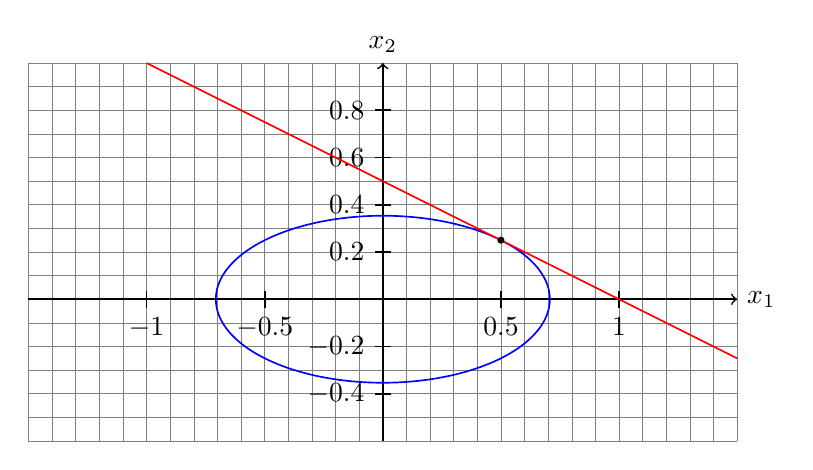
\begin{tikzpicture}[scale=3]
	\draw[very thin,gray,step=1 mm] (-1.5,-0.6) grid (1.5,1);
	\draw[semithick,->] (-1.5,0) -- (1.5,0) node[right] {$x_1$};
	\draw[semithick,->] (0,-0.6) -- (0,1) node[above] {$x_2$};
	\foreach \x in {-1,-0.5,0.5,1}
		\draw[semithick] (\x cm,1pt) -- (\x cm,-1pt) node[anchor=north] {$\x$};
	\foreach \y in {-0.4,-0.2,0.2,0.4,0.6,0.8}
		\draw[semithick] (1pt,\y cm) -- (-1pt,\y cm) node[anchor=east] {$\y$};
	\draw[semithick,blue,smooth cycle,variable=\t,samples=100,domain=-3.1415:3.1415]
		plot({cos(\t r)/sqrt(2)},{sin(\t r)/sqrt(8)});		% r значит радианы
	\draw[semithick,red] (-1,1) -- (1.5,-0.25);				% ограничение
	\fill (0.5,0.25) circle (0.15mm);							% стац. точка
\end{tikzpicture}
\footnotesize \caption{Решение задачи, рассмотренной в четвёртом примере\label{fig:extremum:fourth_example}}
\end{figure}

Задачи оптимизации без ограничений и с ограничениями в форме равенств называются классическими и могут быть решены аналитически. Все остальные (неклассические) очень редко могут решаться аналитически. Для их решения используют алгоритмы Куна-Таккера, градиентные методы, симплексные алгоритмы и методы прямого поиска.

Стационарные точки экстремальной задачи находятся путём решения уравнений вида $ Q(x) = 0 $, рекуррентным методом Ньютона. Последовательные приближения осуществляют по формуле $ x_{n+1} = x_n - \frac{ Q \bigl( x_n \bigr) }{ \Bigl(  dQ \bigl( x_n \bigr) / dx \Bigr) } $, геометрический смысл которой состоит в том, что точка $ x_{n+1} $ вычисляется как пересечение оси абсцисс с касательной к кривой $ y = Q(x) $ в точке $ x_n $.


\begin{problem}
Найти численное значение корня уравнения $ x - \sin x = \frac{ \pi }{2} $.

Составляем рекуррентную формулу $ x_{n+1} = x_n - \frac{ x_n - \sin x_n - \pi/2}{ 1 - \cos x_n } $. При ${{x}_{0}}=2.4$ получается итерационная последовательность $ x_1 = 2.31, x_2 = 2.3099, x_3 = 2.309884, \ldots $ 

\end{problem}


\clearpage
\section{Основы вариационного исчисления\label{variations}}
	\subsection{Оптимизация функционалов\label{variations:general}}

Функционал --- числовая скалярная функция, определяемая на множестве функций: $ y = f(x) $ --- функция от аргумента; $ J(x) = \int\limits_0^T F \left( x, \dot{x}, t \right) \, dt $ --- функция от функций  (скалярная оценка различных функций).

Каждая функция $ x(t) $ является точкой функционального пространства. Пусть эта функция однозначна, непрерывна и дифференцируема на рассматриваемом интервале (такие функции называются гладкими). Если значения функции соответствуют заданным в граничных точках их называют допустимыми. И тогда задача заключается в выборе среди допустимых функций такой, где функционал достигает наименьшего значения $ \underset{ x \in \Omega }{ \min } \, J(x) $. Решением таких задач занимается вариационное исчисление --- аналог дифференциального исчисления для функций.

Итак, для функций условиями экстремума являются:
\begin{gather*}
d \varphi (x) = 0 \quad \to \quad \delta J(x) = 0 \tag{*} \\
d^2 \varphi (x) \underset{\le}{\ge} 0 \quad \to \quad \delta ^2 J(x) \underset{\le}{\ge} 0 \tag{**}
\end{gather*}

Из условия $(*)$ выводится уравнение Эйлера:
\begin{equation}\label{equ:variations:Euler}
\frac{\partial F}{\partial x} - \frac{d}{dt} \left( \frac{\partial F}{\partial \dot{x}} \right) = 0
\end{equation}

Все функции удовлетворяющие этому уравнению, называются экстремалями. Если они проходят через граничные точки, то они называются допустимыми экстремалями.

Из условия $(**)$ выводятся условия Лежандра:
\begin{equation}\label{equ:variations:Legendre}
\frac{\partial ^2 F}{\partial \dot{x} ^2} \underset{\le}{\ge} 0
\end{equation}

\pagebreak

\begin{problem}
$J=\int\limits_0^1 \dot{x}^2 dt \to extr, \quad x(0) = 0, \enskip x(1) = 1 $
\[ F = \dot{x}^2 \enskip \Rightarrow \enskip \frac{\partial F}{\partial x} = 0, \enskip \frac{\partial F}{\partial \dot{x}} = 2\dot{x} \]
Уравнение Эйлера: $ \frac{\partial F}{\partial x} - \frac{d}{dt}\left( \frac{\partial F}{\partial \dot{x}} \right) = 0 \enskip \to \enskip 0 - \frac{d}{dt}\left( 2\dot{x} \right) = 0 $
\[ \ddot{x} = 0, \quad \dot{x} = C_1, \quad x = C_1 t + C_2 \]
\[ \left\{ \begin{darray}{l} x(0) = C_2 = 0 \\ x(1) = C_1 + C_2 = 1 \enskip \Rightarrow \enskip C_1 = 1 \end{darray} \right. \]
Допустимая экстремаль: $\hat{x}=t$\\
Условие Лежандра: $\frac{\partial ^2 F}{\partial \dot{x} ^2} = 2 > 0 \enskip \Rightarrow \enskip \min $
\[ J_{ \min } = \int\limits_0^1 { \left( \dot{\hat{x}} \right) }^2 dt = \int\limits_0^1 { \left( \dot{t} \right) }^2 dt = \int\limits_0^1 1^2 dt = t \Big|_0^1 = 1 \]
\end{problem}
\begin{problem}
Найти уравнение выхода $x(t)$  и характеристический полином СУ, для которой $ J(x) = \int\limits_{0}^{\infty } \left( a_0 x^2 + a_1 \dot{x} ^2 \right) \, dt \enskip \to \enskip \min $, при условиях $ a_0 > 0, a_1 > 0, x(0) = x_0, x( \infty ) = 0 $.
\[ F = a_0 x^2 + a_1 \dot{x} ^2, \quad \frac{\partial F}{\partial x} = 2 a_0 x, \quad \frac{\partial F}{\partial \dot{x}} = 2 a_1 \dot{x} \]
Уравнение Эйлера: $ 2 a_0 x - \frac{d}{dt} \left( 2 a_1 \dot{x} \right) = 0 $
\[ \ddot{x} - \frac{a_0}{a_1}x = 0, \quad \lambda ^2 - \frac{a_0}{a_1} = 0, \quad \lambda _{1, 2} = \pm \sqrt{\frac{a_0}{a_1}} \] 
\[ x(t) = C_1 e^{\sqrt{a_0 / a_1}\,t} + C_2 e^{-\sqrt{a_0 / a_1}\,t} \]
\[ \left. \begin{darray}{l} x(0) = C_1 + C_2 = x_0 \\
		x( \infty ) = C_1 \cdot \infty = 0 \enskip \Rightarrow \enskip C_1 = 0 \end{darray} \right\}
	\enskip \Rightarrow \enskip C_2 = x_0 \]
Допустимая экстремаль: $ \hat{x} = x_0 e^{-\sqrt{a_0 / a_1}\,t} $\\
Условие Лежандра: $\frac{\partial ^2 F}{\partial \dot{x} ^2} = 2 a_1 > 0 \enskip \Rightarrow \enskip \min $\\
Характеристический полином системы: $ D(p) = p + \sqrt{\frac{a_0}{a_1}} $ 
\end{problem}

Обобщим результаты в 2 направлениях:
\begin{itemize}
\item Многомерный случай
\\$X$-векторная функция $={{\left( x_{1}^{\left( t \right)},x_{2}^{\left( t \right)},...x_{n}^{\left( t \right)} \right)}^{T}}$ 
\\$J\left( x \right)=\int\limits_{{{t}_{0}}}^{{{t}_{K}}}{F\left( x,\dot{x},t \right)}dt\to extr$, $\min $;
\\${{x}_{i}}\left( {{t}_{0}} \right)={{x}_{io}}$, ${{x}_{i}}\left( {{t}_{k}} \right)={{x}_{ik}}$
\\Тогда первое необходимое условие (уравнение Эйлера) - система: $\frac{\partial F}{\partial {{x}_{i}}}-\frac{d}{dt}\left( \frac{\partial F}{\partial {{{\dot{x}}}_{i}}} \right)=0,i=\overline{1,n}$ 
\\Второе условие требует анализа матрицы вторых частных производных:
\[\left\| \begin{array}{*{35}{l}}
   \frac{{{\partial }^{2}}F}{\partial \dot{x}_{1}^{2}} & \frac{{{\partial }^{2}}F}{\partial {{{\dot{x}}}_{1}}\partial {{{\dot{x}}}_{2}}} & ... & \frac{{{\partial }^{2}}F}{\partial {{{\dot{x}}}_{1}}\partial {{{\dot{x}}}_{n}}}  \\
   \frac{{{\partial }^{2}}F}{\partial {{{\dot{x}}}_{2}}\partial {{{\dot{x}}}_{1}}} & \frac{{{\partial }^{2}}F}{\partial \dot{x}_{2}^{2}} & ... & \frac{{{\partial }^{2}}F}{\partial {{{\dot{x}}}_{2}}\partial {{{\dot{x}}}_{n}}}  \\
   \frac{{{\partial }^{2}}F}{\partial {{{\dot{x}}}_{n}}\partial {{{\dot{x}}}_{1}}} & \frac{{{\partial }^{2}}F}{\partial {{{\dot{x}}}_{n}}\partial {{{\dot{x}}}_{2}}} & ... & \frac{{{\partial }^{2}}F}{\partial \dot{x}_{n}^{2}}  \\
\end{array} \right\|\]
\\Для \underline{минимума}, все диагональные миноры \underline{должны быть $\ge 0$}, для \underline{$\max \le 0$}. Строгие неравенства дают и \underline{достаточность} условий.
%Непонятно что это пункт или часть случая
\\
\\
\\$J=\int\limits_{0}^{1}{\left( {{x}_{1}}{{x}_{2}}+{{{\dot{x}}}_{1}}{{{\dot{x}}}_{2}} \right)}dt\to extr$, ${{x}_{1}}\left( 0 \right)={{x}_{2}}\left( 0 \right)=1$, ${{x}_{1}}\left( 1 \right)=e$, ${{x}_{2}}\left( 1 \right)=\frac{1}{e}$ 
\\$X=\left( {{x}_{1}},{{x}_{2}} \right)$, $F={{x}_{1}}{{x}_{2}}+{{\dot{x}}_{1}}{{\dot{x}}_{2}}$
\\$\frac{\partial F}{\partial {{x}_{1}}}={{x}_{2}}$ $\frac{\partial F}{\partial {{{\dot{x}}}_{1}}}={{\dot{x}}_{2}}$ $\to $ $\frac{\partial F}{\partial {{x}_{1}}}-\frac{d}{dt}\left( \frac{\partial F}{\partial {{{\dot{x}}}_{1}}} \right)=0$: ${{\ddot{x}}_{2}}-{{x}_{2}}=0$ $\to $ ${{x}_{2}}={{C}_{1}}{{e}^{t}}+{{C}_{2}}{{e}^{-t}}$
\\$\frac{\partial F}{\partial {{x}_{2}}}={{x}_{1}}$, $\frac{\partial F}{\partial {{{\dot{x}}}_{2}}}={{\dot{x}}_{1}}$ $\to$ $\frac{\partial F}{\partial {{x}_{2}}}-\frac{d}{dt}\left( \frac{\partial F}{\partial {{{\dot{x}}}_{2}}} \right)=0$: ${{\ddot{x}}_{1}}-{{x}_{1}}=0$ $\to$ ${{x}_{1}}={{C}_{3}}{{e}^{t}}+{{C}_{4}}{{e}^{-t}}$
\\Подставив начальные и конечные условия получим ${{\hat{x}}_{1}}={{e}^{t}}$, ${{\hat{x}}_{2}}={{e}^{-t}}$
$\left\| \begin{matrix}
   \frac{{{\partial }^{2}}F}{\partial \dot{x}_{1}^{2}} & \frac{{{\partial }^{2}}F}{\partial {{{\dot{x}}}_{1}}\partial {{{\dot{x}}}_{2}}}  \\
   \frac{{{\partial }^{2}}F}{\partial {{{\dot{x}}}_{2}}\partial {{{\dot{x}}}_{1}}} & \frac{{{\partial }^{2}}F}{\partial \dot{x}_{2}^{2}}  \\
\end{matrix} \right\|=\left\| \begin{matrix}
   0 & 1  \\
   1 & 0  \\
\end{matrix} \right\|$ $\to $  ${{\Delta }_{1}}=0$, ${{\Delta }_{2}}=-1$ $\to $ имеет место \underline{$\max $}
\\${{J}_{\max }}=\int\limits_{0}^{1}{\left( {{e}^{t}}{{e}^{-t}}+{{e}^{t}}\left( {{e}^{-t}} \right) \right)}dt=0$
\item Задача со старшими производными:
\\$J\left( x \right)=\int\limits_{{{t}_{0}}}^{{{t}_{k}}}{F\left( x,\dot{x},\ddot{x},...\overset{n}{\mathop{x}}\,,t \right)}dt$
\\$x\left( {{t}_{0}} \right)={{x}_{0}},\dot{x}\left( {{t}_{0}} \right)={{x}_{0}},...\overset{\left( n-1 \right)}{\mathop{x}}\,\left( {{t}_{0}} \right)=\overset{\left( n-1 \right)}{\mathop{{{x}_{0}}}}\,$
\\$x\left( {{t}_{k}} \right)={{x}_{0}},\dot{x}\left( {{t}_{k}} \right)={{x}_{k}},...\overset{\left( n-1 \right)}{\mathop{x}}\,\left( {{t}_{k}} \right)=\overset{\left( n-1 \right)}{\mathop{{{x}_{k}}}}\,$
Существует 2 способа решения:
\begin{enumerate}
\item Рассматривается векторная функция, составляемая из исходной $x\left( t \right)$ и её $\left( n-1 \right)$ производной - т.е. задача, как многомерный случай
\item Уравнение Эйлера преобразуется в уравнение Эйлера-Пуассона:
$\frac{\partial F}{\partial x}-\frac{d}{dt}\left( \frac{\partial F}{\partial \dot{x}} \right)+\frac{{{\partial }^{2}}}{\partial {{t}^{2}}}\left( \frac{\partial F}{\partial \ddot{x}} \right)-...+{{\left( -1 \right)}^{n}}\frac{{{d}^{n}}}{d{{t}^{n}}}\left( \frac{\partial F}{\partial \overset{\left( n \right)}{\mathop{x}}\,} \right)=0$,
\\Условие Лежандра: $\frac{{{\partial }^{2}}F}{{{\left( \partial \overset{\left( n \right)}{\mathop{x}}\, \right)}^{2}}}\ne 0$
\\ $J\left( x \right)=\int\limits_{0}^{1}{{{{\ddot{x}}}^{2}}}dt\to extr$, $x\left( 0 \right)=\dot{x}\left( 0 \right)=0$, $x\left( 1 \right)=0$, $\dot{x}\left( 1 \right)=1$
\\$F={{\ddot{x}}^{2}}$: $\frac{\partial F}{\partial x}-\frac{d}{dt}\left( \frac{\partial F}{\partial \dot{x}} \right)+\frac{{{\partial }^{2}}}{\partial {{t}^{2}}}\left( \frac{\partial F}{\partial \ddot{x}} \right)=0$
\\$0-0+\frac{{{\partial }^{2}}}{\partial {{t}^{2}}}\left( 2\ddot{x} \right)=0$ $\to $ $\overset{\left( 4 \right)}{\mathop{x}}\,=0$, $\overset{\left( 3 \right)}{\mathop{x}}\,={{C}_{1}}$, $\overset{\left( 2 \right)}{\mathop{x}}\,={{C}_{1}}t+{{C}_{2}}$, $\dot{x}=\frac{1}{2}{{C}_{1}}{{t}^{2}}+{{C}_{2}}t+{{C}_{3}}$
\\$x=\frac{1}{6}{{C}_{1}}{{t}^{3}}+\frac{1}{2}{{C}_{2}}{{t}^{2}}+{{C}_{3}}t+{{C}_{4}}$, 
\\$t\left( 0 \right):\,0={{C}_{4}},\,0={{C}_{3}}$
\\$t\left( 1 \right):\frac{1}{6}{{C}_{1}}+\frac{1}{2}{{C}_{2}}=0,\frac{1}{2}{{C}_{1}}+{{C}_{2}}=0$ $\to $ ${{C}_{1}}=6,\,{{C}_{2}}=-2$
\\$\hat{x}={{t}^{3}}-{{t}^{2}}$, $\ddot{\hat{x}}=6t-2$ 
\\${{J}_{\min }}=\int\limits_{0}^{1}{{{\left( 6t-2 \right)}^{2}}}dt=\left. 12{{t}^{3}} \right|_{0}^{1}-\left. 12{{t}^{2}} \right|_{0}^{1}+\left. 4t \right|_{0}^{1}=4$
\end{enumerate}
\end{itemize}
	\subsection{Задачи с нефиксированными границами\label{variations:floating_ends}}
Как для начального момента времени (левого конца) так и для конечного момента времени (правого конца) могут быть следующие варианты: (для удобства все примеры для правого конца)


\begin{itemize}
\item Задача со свободным правым концом ${{t}_{k}}=\operatorname{var}$, $x\left( {{t}_{k}} \right)=\operatorname{var}$
\item Задача с подвижным правым концом ${{t}_{k}}=T$, $x\left( {{t}_{k}} \right)=\operatorname{var}$
\item Задача со скользящим правым концом ${{t}_{k}}=T$-не задано, $x\left( {{t}_{k}} \right)$ не задано, но определена их взаимосвязь $\psi \left( t \right)$
\end{itemize}
\par В этих случаях (когда отсутствует соответствующее граничное условие) необходимым условием экстремума, кроме уравнения Эйлера $\frac{\partial F}{\partial x}-\frac{d}{dt}\left( \frac{\partial F}{\partial \dot{x}} \right)=0$, становятся \underline{условия трансверсальности}:
\\$\left\{ \begin{array}{*{35}{l}}
   {{\left. \left( F-\frac{\partial F}{\partial \dot{x}}\dot{x} \right) \right|}_{{{t}_{k}}}}=0$ - если не задано ${{t}_{k}}$ и $x\left( {{t}_{k}} \right)$  
   $\\{{\left. \frac{\partial F}{\partial \dot{x}} \right|}_{{{t}_{k}}}}=0$ - если не задано $x\left( {{t}_{k}} \right)$
   $\\{{\left. \left( F-\frac{\partial F}{\partial \dot{x}}\left( \dot{x}-\dot{\psi } \right) \right) \right|}_{{{t}_{k}}}}=0$ - если конец скользящий   
$\end{array} \right.$
\\В векторном случае: $X=\left( {{x}_{1}}\left( t \right),{{x}_{2}}\left( t \right)...{{x}_{n}}\left( t \right) \right)$ необходимым условием достижения экстремума является система уравнений:
\\$\left\{ \begin{array}{*{35}{l}}
   \frac{\partial F}{\partial {{x}_{i}}}-\frac{d}{dt}\left( \frac{\partial F}{\partial {{x}_{i}}} \right)=0,\,i=\overline{1,n}$ - уравнение Эйлера   
   $ \\   {{\left. \left( F-\sum\limits_{i=1}^{n}{\frac{\partial F}{\partial {{{\dot{x}}}_{i}}}{{{\dot{x}}}_{i}}} \right) \right|}_{{{t}_{0}}}}=0;\,\,{{\left. \left( F-\sum\limits_{i=1}^{n}{\frac{\partial F}{\partial {{{\dot{x}}}_{i}}}{{{\dot{x}}}_{i}}} \right) \right|}_{{{t}_{k}}}}=0$ 
   $\\{{\left. \frac{\partial F}{\partial {{{\dot{x}}}_{i}}} \right|}_{{{t}_{0}}}}=0,\,i=\overline{1,n};\,\,{{\left. \frac{\partial F}{\partial {{{\dot{x}}}_{i}}} \right|}_{{{t}_{k}}}}=0,\,i=\overline{1,n}$ 
$\\\end{array} \right.$
\\Вторая и третья строки системы условия трансверсальности с соответвующим незаданным граничным условием.
\\Максимальное количество условий трансверсальности $2n+2$.
\\
\\
\ExampleMy 
\begin{itemize}
\item $J=\int\limits_{0}^{1}{\left( {{{\dot{x}}}^{2}}+x \right)dt}\to extr$, $x\left( 1 \right)=0$
\\$\frac{\partial F}{\partial x}=1$, $\frac{\partial F}{\partial \dot{x}}=2\dot{x}$, уравнение Эйлера: $1-\frac{d}{dt}\left( 2\dot{x} \right)=0$ условие трансверсальности: $2\dot{x}\left( 0 \right)=0$
\\Решаем: $1-2\ddot{x}=0$, $\,\ddot{x}=\frac{1}{2}$, $\dot{x}\left( t \right)=\frac{t}{2}+{{C}_{1}}$,$x\left( t \right)=\frac{{{t}^{2}}}{4}+{{C}_{1}}+{{C}_{2}}$
\\$x\left( 0 \right)={{C}_{1}}=0$, $x\left( 1 \right)=\frac{1}{4}+{{\not{C}}_{1}}+{{C}_{2}}=0\to {{C}_{2}}=-\frac{1}{4}$, $\hat{x}\left( t \right)=\frac{1}{4}\left( {{t}^{2}}-1 \right)$ - допустимая экстремаль.  
$\frac{{{\partial }^{2}}F}{\partial {{{\dot{x}}}^{2}}}=2>0$ - \underline{min}: ${{J}_{\min }}=\int\limits_{0}^{1}{\left( \frac{1}{4}{{t}^{2}}+\frac{1}{4}\left( {{t}^{2}}-1 \right) \right)dt=-\frac{1}{12}}$ 
\end{itemize}
Подводя итог хотелось бы ответить, что необходимое условия минимизации функционалов представляются дифференциальными уравнениями относительно неизвестной функции (при минимизации функций $\to $ необходимое условие - алгебраические уравнения). Причём можно показать, что это нелинейное дифференциальное уравнение II порядка:
\\$\frac{\partial F}{\partial x}-\frac{d}{dt}\left( \frac{\partial F}{\partial \dot{x}} \right)=0$, $\frac{d}{dt}\left( \frac{\partial F}{\partial \dot{x}} \right)=\frac{\partial }{\partial t}\frac{\partial F}{\partial \dot{x}}+\frac{\partial }{\partial x}\left( \frac{dx}{dt}\frac{\partial F}{\partial \dot{x}} \right)+\frac{\partial }{\partial \dot{x}}\left( \frac{dx}{dt}\frac{\partial F}{\partial \dot{x}} \right)$, $\frac{\partial F}{\partial \dot{x}}=\frac{\partial F}{\partial \dot{x}}\left( t,x,\dot{x} \right)$
\\Тогда: \[\frac{\partial F}{\partial x}-\frac{\partial }{\partial t}\frac{\partial F}{\partial \dot{x}}-\frac{{{\partial }^{2}}F}{\partial \dot{x}\partial \dot{x}}\dot{x}-\frac{{{\partial }^{2}}F}{\partial {{{\dot{x}}}^{2}}}\ddot{x}=0\]
\\Уравнение Эйлера может приобретать вид:
\begin{itemize}
\item Если $F\left( x,t \right)$, не зависит от $\dot{x}$ $\to $ $\frac{\partial F}{\partial x}=0$
\item Если $F\left( \dot{x},t \right)$, не зависит от $x$ $\to $ $\frac{\partial F}{\partial \dot{x}}=const$ 
\item Если $F\left( x,\dot{x} \right)$, не зависит от $t$ $\to $ $F-\dot{x}\frac{\partial F}{\partial \dot{x}}=const$
\end{itemize}

	\subsection{Оптимизация функционалов с ограничениями в форме равенств\label{variations:conditional_extremum}}
\par При решении различных технических проблем нахождение экстремума требует учёта связей в форме алгебраических, дифференциальных и интегральных уравнений, т.е. дополнительных условий. Тогда вместо функции $F\left( x,t \right)$ берётся функция $L\left( x,u,t,\lambda  \right)=F\left( x,\dot{x},t \right)+{{\lambda }^{T}}\left( t \right)\centerdot \Phi \left( x,u,t \right)$ - Лагранжиан и уравнение приобретает вид Эйлера-Лагранжа:
\\$\left\{ \begin{array}{*{35}{l}}
   \frac{\partial L}{\partial x}-\frac{d}{dt}\left( \frac{\partial L}{\partial \dot{x}} \right)=0$, где $\lambda \left( t \right)$ - вектор множителей Лагранжа,   
   $\\\frac{\partial L}{\partial u}-\frac{d}{dt}\left( \frac{\partial L}{\partial \dot{u}} \right)=0$    зависящий от времени.
   $\\\end{array} \right.$
\\
\\\ExampleMy Пусть произвольная динамическая система 
\\$\left\{ \begin{array}{*{35}{l}}
   {{{\dot{x}}}_{1}}={{x}_{2}}  \\
   {{{\dot{x}}}_{2}}=-{{x}_{1}}+u  \\
\end{array} \right.$
с начальными состоянием $\left| \begin{array}{*{35}{l}}
   {{x}_{1}}\left( 0 \right)  \\
   {{x}_{2}}\left( 0 \right)  \\
\end{array} \right|$
и нулевым конечным $\left| \begin{array}{*{35}{l}}
   {{x}_{1}}\left( \infty  \right)=0  \\
   {{x}_{2}}\left( \infty  \right)=0  \\
\end{array} \right|$ доставляет $\min \int\limits_{0}^{\infty }{\left( x_{1}^{2}+x_{2}^{2}+0.1{{u}^{2}} \right)dt}$
Для решения:
\begin{enumerate}
\item Составляем Лагранжиан:
$L\left( x,u,\lambda  \right)=\left( x_{1}^{2}+x_{2}^{2}+0.1{{u}^{2}} \right)+{{\lambda }_{1}}\left( {{{\dot{x}}}_{1}}-{{x}_{2}} \right)+{{\lambda }_{2}}\left( {{{\dot{x}}}_{2}}+{{x}_{1}}-u \right)$
\item Составляем уравнение Эйлера-Лагранжа:
\\$\frac{\partial L}{\partial {{x}_{1}}}-\frac{d}{dt}\left( \frac{\partial L}{\partial {{{\dot{x}}}_{1}}} \right)=0$; $2{{x}_{1}}+{{\lambda }_{2}}-\frac{d}{dt}\left( {{\lambda }_{1}} \right)$
\\$\frac{\partial L}{\partial {{x}_{2}}}-\frac{d}{dt}\left( \frac{\partial L}{\partial {{{\dot{x}}}_{2}}} \right)=0$; $2{{x}_{2}}-{{\lambda }_{1}}-\frac{d}{dt}\left( {{\lambda }_{2}} \right)$
\\$\frac{\partial L}{\partial u}-\frac{d}{dt}\left( \frac{\partial L}{\partial \dot{u}} \right)=0$; $0.1\cdot 2u-{{\lambda }_{2}}$ 
Учитывая уравнение системы и исключая получим:
$\begin{array}{*{35}{l}}
   {{{\dot{x}}}_{1}}={{x}_{2}},\,\,{{{\dot{x}}}_{2}}=-{{x}_{1}}+5{{\lambda }_{2}}  \\
   {{{\dot{\lambda }}}_{1}}=2{{x}_{1}}+{{\lambda }_{2}},\,\,{{{\dot{\lambda }}}_{2}}=-{{\lambda }_{1}}+2{{x}_{2}}  \\
\end{array}$, т.е. $\left| \begin{matrix}
   {{{\dot{x}}}_{1}}  \\
   {{{\dot{x}}}_{2}}  \\
   {{{\dot{\lambda }}}_{1}}  \\
   {{{\dot{\lambda }}}_{2}}  \\
\end{matrix} \right|=\underbrace{\left| \begin{matrix}
   0 & 1 & 0 & 0  \\
   -1 & 0 & 0 & 5  \\
   2 & 0 & 0 & 1  \\
   0 & 2 & -1 & 0  \\
\end{matrix} \right|}_{A}\left| \begin{matrix}
   {{x}_{1}}  \\
   {{x}_{2}}  \\
   {{\lambda }_{1}}  \\
   {{\lambda }_{2}}  \\
\end{matrix} \right|$
\\$\left| Ep-A \right|=\left| \begin{matrix}
   p & -1 & 0 & 0  \\
   1 & p & 0 & -5  \\
   -2 & 0 & p & -1  \\
   0 & -2 & -1 & p  \\
\end{matrix} \right|={{p}^{4}}-8{{p}^{2}}+11$
\\${{p}_{1,2}}=\pm 2.5$, ${{p}_{3,4}}=\pm 1.32$
\\${{z}^{2}}-8z+11$, ${{z}_{1,2}}=4\pm \sqrt{16-11}=\left\{ \begin{array}{*{35}{l}}
   6.25  \\
   1.75  \\
\end{array} \right.$
\par Зная, что условию устойчивого решения отвечают только левые корни ищем решение в форме 
\\${{x}_{_{1}}}\left( t \right)={{C}_{1}}\exp \left( -2.5t \right)+{{C}_{2}}\exp \left( -1.32t \right)+\underbrace{{{C}_{3}}\exp \left( 2.5t \right)+{{C}_{4}}\exp \left( 1.32t \right)}_{x\left( \infty  \right)=0}$
\\${{x}_{2}}={{\dot{x}}_{1}}=-2.5{{C}_{1}}\exp \left( -2.5t \right)-1.32{{C}_{2}}\exp \left( -1.32t \right)$
\\$u={{\dot{x}}_{2}}+{{x}_{1}}=6.25{{C}_{1}}\exp \left( -2.5t \right)+1.75{{C}_{2}}\exp \left( -1.32t \right)-2.5{{C}_{1}}\exp \left( -2.5t \right)-1.32{{C}_{2}}\exp \left( -1.32t \right)=3.75{{C}_{1}}\exp \left( -2.5t \right)+0.43{{C}_{2}}\exp \left( -1.32t \right)$
\\Зная:
\\$\left| \begin{array}{*{35}{l}}
   {{x}_{1}}  \\
   {{x}_{2}}  \\
\end{array} \right|=\left| \begin{matrix}
   1 & 1  \\
   -2.5 & -1.32  \\
\end{matrix} \right|\left| \begin{array}{*{35}{l}}
   {{C}_{1}}\exp \left( -2.5t \right)  \\
   {{C}_{2}}\exp \left( -1.32t \right)  \\
\end{array} \right|$
$\to $
$\left| \begin{array}{*{35}{l}}
   {{C}_{1}}\exp \left( -2.5t \right)  \\
   {{C}_{2}}\exp \left( -1.32t \right)  \\
\end{array} \right|=\left| \begin{matrix}
   -1.12 & -0.85  \\
   2.12 & 0.85  \\
\end{matrix} \right|\left| \begin{array}{*{35}{l}}
   {{x}_{1}}  \\
   {{x}_{2}}  \\
\end{array} \right|$
\\${{x}_{1}}=a+b$ $a={{x}_{1}}-b\to {{x}_{2}}=-2.5\left( {{x}_{1}}-b \right)-1.32b=-2.5{{x}_{1}}+1.17b\to b\approx 2.12{{x}_{1}}+0.85{{x}_{2}}$
\\${{x}_{2}}=-2.5a-1.32b$ $a={{x}_{1}}-b={{x}_{1}}-2.12{{x}_{1}}-0.85{{x}_{2}}=1.12{{x}_{1}}-0.85{{x}_{2}}$
\\$u=\left( 3.75;\,\,0.43 \right)\left( \begin{matrix}
   -1.12 & -0.85  \\
   2.12 & 0.85  \\
\end{matrix} \right)\left( \begin{matrix}
   {{x}_{1}}  \\
   {{x}_{2}}  \\
\end{matrix} \right)=-3.2{{x}_{1}}-2.8{{x}_{2}}$
\end{enumerate}
	\subsection{Каноническая (Гамильтонова) форма уравнений Эйлера (Лагранжа)\label{variations:Canonical_Euler}}
Стремление избавится от двойного дифференцирования (по времени и производны  $\frac{\partial }{\partial \dot{x}}$,$\frac{\partial }{\partial \dot{u}}$ - состояния и управления) привело к предложению ввести канонические переменные ${{\psi }_{i}}\left( t \right)$ сопряжённые с переменными состояния ОУ и функцию Гамильтона: $H=-F\left( x,u,t \right)+\sum\limits_{i=1}^{n}{{{\psi }_{i}}{{{\dot{x}}}_{i}}}=-L\left( x,u,\lambda ,t \right)+\sum\limits_{i=1}^{n}{{{\psi }_{i}}{{{\dot{x}}}_{i}}}$, где ${{\psi }_{i}}=\frac{\partial F}{\partial {{{\dot{x}}}_{i}}}$ или $\frac{\partial L}{\partial {{{\dot{x}}}_{i}}}$, и тогда можно получить, учитывая что $\frac{\partial H}{\partial {{x}_{i}}}=-\frac{\partial F}{\partial {{x}_{i}}}=-\frac{\partial L}{\partial {{x}_{i}}}$ ${{\dot{x}}_{i}}=\frac{d{{{\dot{x}}}_{i}}}{dt}=\frac{\partial H}{\partial {{\psi }_{i}}}$ $\frac{\partial F}{\partial {{x}_{i}}}-\frac{d}{dt}\underbrace{\left( \frac{\partial F}{\partial {{{\dot{x}}}_{i}}} \right)}_{{{\psi }_{i}}}\to \frac{d}{dt}{{\psi }_{i}}=\frac{\partial F}{\partial {{x}_{i}}}$, систему
$\left\{ \begin{array}{*{35}{l}}
   \frac{d{{x}_{i}}}{dt}=\frac{\partial H}{\partial {{\psi }_{i}}},\,i=\overline{1,n}  \\
   \frac{d{{\psi }_{i}}}{dt}=-\frac{\partial H}{\partial {{x}_{i}}},\,i=\overline{1,n}  \\
   \frac{dH}{d{{u}_{j}}}=0,\,\,j=\overline{1,m}  \\
\end{array} \right.$
\\Учитывая, что в уравнении ОУ ($\dot{x}=Ax+Bu$) отсутствует производные управления ($\dot{u}$). При не фиксированных граничных условиях уравнение трансверсальности в канонической форме имеет вид: 
\[\begin{array}{*{35}{l}}
   {{\psi }_{i}}\left( {{t}_{0}} \right)=0,{{\psi }_{i}}\left( {{t}_{k}} \right)=0  \\
   H\left( {{t}_{0}} \right)=0,H\left( {{t}_{k}} \right)=0  \\
\end{array}\]
\par Такая форма уравнений даёт большое преимущество, т.к. слева только дифференциирование по времени, а справа частные производные по времени.
\par Для общей задачи Лагранжа канонические переменные $\psi \left( t \right)$ совпадают с неизвестными множителями Лагранжа $\lambda \left( t \right)$.
\par Кроме того, переход к функции Гамильтона позволит снизить требования к гладкости изменения переменных состояния и управления и решать задачи в условиях ограничений в виде неравенства.
\par Для консервативных механических систем функция Гамильтона $H$ имеет простой физический смысл - она совпадает с полной механической энергией $H=const$ - имеет смысл закона сохранения полной механической энергии.
\par В общем случае для линейного объекта в форме уравнений состояния $\dot{x}=Ax+Bu$ ($n$-размерности) отсутствует зависимость от $\dot{u}$ уравнения вариационной задачи записываются в следующем виде:
Из $extrJ=\int\limits_{0}^{\infty }{F\left( x,u,t \right)dt}$
$L\left( \dot{x},u,t,\lambda  \right)=F\left( x,u,t \right)+{{\lambda }^{T}}\left( t \right)\cdot \Phi \left( x,u,t \right)$ $\Phi \left( x,u,t \right)=\dot{x}-Ax-Bu$
\\$H\left( {} \right)={{\lambda }^{T}}\left( t \right)\dot{x}-L\left( x,u,t,\lambda  \right)=-F\left( x,u,t \right)+{{\lambda }^{T}}\left( t \right)\cdot \left( \dot{x}-\dot{x}\underbrace{+Ax+Bu}_{{{\Phi }_{1}}\left( x,u,t \right)} \right)$
получается система 
\\$\left\{ \left. \begin{array}{*{35}{l}}
   \frac{\partial X}{\partial t}=\left\| \frac{\partial H}{\partial {{\lambda }_{i}}} \right\|=AX+BU,\,\,i=\overline{1,n}  \\
   \frac{\partial \lambda }{\partial t}=-\left\| \frac{\partial H}{\partial {{x}_{i}}} \right\|=\left\| \frac{\partial F}{\partial {{x}_{i}}} \right\|+{{\lambda }^{T}}\left\| \frac{\partial {{\Phi }_{1}}}{\partial {{x}_{i}}} \right\|,\,\,\,i=\overline{1,n}  \\
   \frac{\partial H}{\partial {{u}_{j}}}=\frac{\partial F}{\partial {{u}_{j}}}+\sum\limits_{i=1}^{n}{{{\lambda }_{i}}\frac{\partial {{\varphi }_{1i}}}{\partial {{u}_{j}}}}=0,\,\,j=\overline{1,r}  \\
\end{array} \right\} \right.2n+r$ уравнений
\\
\ExampleMy Определим оптимальное управление объектом:
\\$T\dot{x}+x=ku$, $\frac{x}{u}=\frac{k}{Tp+1}\to \dot{x}=-\frac{1}{T}x+\frac{k}{T}u=ax+bu$
\\$J=\int\limits_{0}^{\infty }{\left( q{{x}^{2}}+r{{u}^{2}} \right)}dt,\to L=q{{x}^{2}}+r{{u}^{2}}+\lambda \left( \dot{x}-ax-bu \right),\,H=-q{{x}^{2}}-r{{u}^{2}}+\lambda \left( ax+bu \right)$
\\$\left\{ \begin{array}{*{35}{l}}
   \dot{x}=\frac{\partial H}{\partial \lambda }=ax+bu  \\
   \dot{\lambda }=-\frac{\partial H}{\partial x}=-\left( 2qx+\lambda a \right)=2qx-\lambda a  \\
   0=-\frac{\partial H}{\partial u}=-\left( -2ru+\lambda b \right)=2ru-\lambda b  \\
\end{array} \right.$ $\to u=\frac{b}{2r}\lambda $
\\Имеем систему уравнений:
\\$\left\{ \begin{array}{*{35}{l}}
   \dot{x}=ax+\frac{{{b}^{2}}}{2r}\lambda   \\
   \dot{\lambda }=2qx-a\lambda   \\
\end{array} \right.=\left| \begin{matrix}
   a & \frac{{{b}^{2}}}{2r}  \\
   2q & -a  \\
\end{matrix} \right|\left| \begin{matrix}
   x  \\
   \lambda   \\
\end{matrix} \right|$
\\Для определения корней системы составим определитель
\\$\Delta \left( p \right)=\left| Ep-A \right|=\left| \begin{matrix}
   p-a & -\frac{{{b}^{2}}}{2r}  \\
   -2q & p+a  \\
\end{matrix} \right|={{p}^{2}}-{{a}^{2}}-2q\left( \frac{{{b}^{2}}}{2r} \right)={{p}^{2}}-\left( {{a}^{2}}+q\frac{{{b}^{2}}}{r} \right)=0$
\\${{p}_{1,2}}=\pm \sqrt{{{a}^{2}}+\frac{q{{b}^{2}}}{r}}$-условию устойчивости удовлетворяет только отрицательный корень, поэтому решение ищем в виде $\left\{ \begin{array}{*{35}{l}}
   x={{C}_{1}}\exp \left( {{p}_{2}}t \right)  \\
   \lambda ={{C}_{2}}\exp \left( {{p}_{2}}t \right)  \\
\end{array} \right.$ ${{C}_{1}},\,{{C}_{2}}$ - постоянные интегрирования ${{C}_{1}}={{x}_{0}}$, ${{C}_{2}}=\frac{\left( {{p}_{2}}-a \right)2r}{b}{{C}_{1}}=\frac{2q}{{{p}_{2}}+a}{{C}_{1}}$
\\Следовательно искомое оптимальное уравнение
\\${{U}_{}}\left( t \right)=\frac{b}{2r}\lambda \left( t \right)=\frac{bq}{r\left( {{p}_{2}}-a \right)}\cdot \underbrace{{{C}_{1}}\exp \left( {{p}_{2}}t \right)}_{x\left( t \right)}=u\left( t \right)\to \underbrace{\frac{{{p}_{2}}-a}{b}}_{{{K}_{}}}x\left( t \right)$ - такое решение определяет структуру оптимального регулятора в форме отрицательной обратной связи
\\${{K}_{}}=\frac{{{p}_{2}}-a}{b}=-\frac{a+\sqrt{{{a}^{2}}+q\frac{{{b}^{2}}}{r}}}{b}$   
\par Вспомним пример поиска характеристического полинома системы $D\left( p \right)=p+\sqrt{\frac{{{a}_{0}}}{{{a}_{1}}}}$ доставляющего $\min J=\int\limits_{0}^{\infty }{\left( q{{x}^{2}}+q{{{\dot{x}}}^{2}} \right)}dt$ перепишем в нашем случае:
\\$J=\int\limits_{0}^{\infty }{\left( q{{x}^{2}}+r{{u}^{2}} \right)}dt=\int\limits_{0}^{\infty }{\left( q{{x}^{2}}+r{{\left( \frac{\dot{x}-ax}{b} \right)}^{2}} \right)}dt=\int\limits_{0}^{\infty }{\left( \left( q+r\frac{{{a}^{2}}}{{{b}^{2}}} \right){{x}^{2}}-\frac{2ra}{{{b}^{2}}}x\dot{x}+\frac{r}{{{b}^{2}}}{{{\dot{x}}}^{2}} \right)}dt$
\\$F=\left( q+r\frac{{{a}^{2}}}{{{b}^{2}}} \right){{x}^{2}}-\frac{2ra}{{{b}^{2}}}x\dot{x}+\frac{r}{{{b}^{2}}}{{\dot{x}}^{2}}\to \frac{\partial F}{\partial x}=2\left( q+r\frac{{{a}^{2}}}{{{b}^{2}}} \right)x-\frac{2ra}{{{b}^{2}}}\dot{x}$
\\$\frac{\partial F}{\partial \dot{x}}=-\frac{2ra}{{{b}^{2}}}x+\frac{2r}{{{b}^{2}}}\dot{x}$, уравнение Эйлера:
\\$\frac{\partial F}{\partial x}-\frac{d}{dt}\left( \frac{\partial F}{\partial \dot{x}} \right)=0\to 2\left( q+r\frac{{{a}^{2}}}{{{b}^{2}}} \right)x-\frac{2ra}{{{b}^{2}}}\dot{x}+\frac{2ra}{{{b}^{2}}}\dot{x}-\frac{2ra}{{{b}^{2}}}\ddot{x}\to \ddot{x}-\left( {{a}^{2}}+q\frac{{{b}^{2}}}{r} \right)x=0$
\\Соответствующий характеристический полином ${{p}^{2}}-\left( {{a}^{2}}+q\frac{{{b}^{2}}}{r} \right)=0$ можно представить как $\left[ {{p}^{2}}-\sqrt{{{a}^{2}}+q\frac{{{b}^{2}}}{r}} \right]\left[ {{p}^{2}}+\sqrt{{{a}^{2}}+q\frac{{{b}^{2}}}{r}} \right]=0$ - произведение полиномов с симметричным расположением левого и правого полюсов - это \underline{факторизация}. Устойчивый характер процессов дает полином ${{p}^{2}}+\sqrt{{{a}^{2}}+q\frac{{{b}^{2}}}{r}}=0$.
\par Если мы ищем оптимальную обратную пропорциональную связь для объекта $\dot{x}=ax+bu$, то ${{U}_{opt}}={{K}_{opt}}\cdot x$ $\dot{x}=ax+b{{K}_{oc}}x=\left( a+b{{K}_{oc}} \right)x$ и $D\left( p \right)=p-\left( a+b{{K}_{oc}} \right)$. Приравнивая два полинома 
$p+\sqrt{{{a}^{2}}+q\frac{{{b}^{2}}}{r}}=p-\left( a+b{{K}_{oc}} \right)$, получим ${{K}_{oc}}=\frac{-\sqrt{{{a}^{2}}+q\frac{{{b}^{2}}}{r}}-a}{b}$ - как видно решения совпадают - в литературе принято такой подход называть синтезом линейного оптимального регулятора в частотной области.
\\Записывая факторизацию для $D\left( p \right)\to \left[ p-\left( a+b{{K}_{oc}} \right) \right]\left[ p+\left( a+b{{K}_{oc}} \right) \right]={{p}^{2}}-\left( {{a}^{2}}+q\frac{{{b}^{2}}}{r} \right)$ получим ${{p}^{2}}-{{\left( a+b{{K}_{oc}} \right)}^{2}}={{p}^{2}}-\left( {{a}^{2}}+\frac{{{b}^{2}}}{r}q \right)$ - уравнение $K_{oc}^{2}+\frac{2a}{b}{{K}_{oc}}-\frac{q}{r}=0$ откуда:  ${{K}_{oc}}=-\frac{a}{b}\pm \sqrt{\frac{{{a}^{2}}}{{{b}^{2}}}+\frac{q}{r}}$ скалярное стационарное уравнение Риккати.

\clearpage
\section{Принцип максимума\label{maximum}}
	\subsection{Определение\label{maximum:def}}
\par В целом ряде практических задач оптимизация функционала при заданных дифференциальных (динамических) уравнениях объекта $\left\{ \dot{X}=\Phi \left( x,u \right)=AX+BU \right\}$ требуется обеспечивать при ограниченных диапазонах допустимого изменения управлений $\left| {{u}_{i}} \right|\le {{U}_{i}}$   и/или координат объекта $\left| {{x}_{i}} \right|\le {{X}_{i}}$. В изменениях функций образуются переломы, в изменении производных разрыва. Нарушаются условия, при которых были выведены уравнения Эйлера и Эйлера-Лагранжа в вариациях.
\par Коллективом ученых под руководством академика Л.С.Понтрягина (В.Г.Болтянский,Р.В.Гамкрелидзе,Е.Ф.Мищенко и др.) был разработан принцип максимума, использующий понятие игольчатой вариации относительно оптимального управления и траектории движения, что позволило доказать применимость модифицированной функции Гамильтона для таких неклассических вариационных задач. Модификация заключалась в следующем:
\begin{itemize}
\item Уравнение для критерия качества $J=\int\limits_{{{t}_{0}}}^{{{t}_{K}}}{{{F}_{0}}\left( x,u \right)dt}$ из интегральной формы преобразовывалось в дифференциальную ${{\dot{x}}_{0}}={{\dot{F}}_{0}}\left( x,u \right)$, ${{x}_{0}}=\left. J \right|_{{{t}_{0}}}^{{{t}_{k}}}$
\item Формирования расширенного вектора ${{\left[ {{x}_{0}},x \right]}_{n+1}}$ и новой функции Гамильтона ${{H}^{*}}\left( {{\psi }_{0}},\psi ,x,u \right)={{\psi }_{0}}{{F}_{0}}\left( x,u \right)+{{\psi }^{T}}\Phi \left( x,u \right)=\sum\limits_{i=0}^{n}{{{\psi }_{i}}{{f}_{i}}\left( x,U \right)}$, где ${{\psi }_{0}}=-1$ для перехода об минимизации $J$ к максимизации $H$.
Канонические уравнения Гамильтона тогда имеют вид:
$\left\{ \begin{array}{*{35}{l}}
   \frac{d{{x}_{i}}}{dt}=\frac{\partial {{H}^{*}}}{\partial {{\psi }_{i}}},\,\,i=\overline{0,n}  \\
   \frac{\partial {{\psi }_{i}}}{dt}=-\frac{\partial {{H}^{*}}}{\partial {{x}_{i}}},\,\,i=\overline{0,n}  \\
   \frac{\partial {{H}^{*}}}{\partial U}=0  \\
\end{array} \right.$, их количество $2n+2+r$ и решение задачи при фиксированных начальной $x\left( {{t}_{0}} \right)$ и конечной $x\left( {{t}_{k}} \right)$ точках дается теоремой (без доказательства).
\end{itemize}
\underline{Теорема (Л.С.Понтягин,1956 г)} Для того, чтобы допустимое управление ${{u}^{*}}\left( t \right)$ и соответствующая ему траектория ${{x}^{*}}\left( t \right)$ были оптимальными \underline{необходимо} существование такой ненулевой непрерывной векторной функции ${{\psi }^{*}}\left( t \right)$, отвечающей в силу уравнений Гамильтона функциям  ${{u}^{*}}\left( t \right)$ и ${{x}^{*}}\left( t \right)$, что:
\begin{enumerate}
\item В $\forall $ момент времени, когда ${{u}^{*}}\left( t \right)$ непрерывна при ${{t}_{0}}\le t\le {{t}_{k}}$ функция ${{H}^{*}}\left( {{x}^{*}},{{u}^{*}} \right)=\underset{u\in U}{\mathop{\max }}\,{{H}^{*}}\left( \psi _{0}^{*},{{\psi }^{*}},{{x}^{*}},u \right)$ - достигает максимума.
\item В $\forall $ момент времени $\psi _{0}^{*}=-1$,${{H}^{*}}\left( {{\psi }^{*}}\left( T \right),{{x}^{*}}\left( T \right) \right)=0$
\end{enumerate}
При этом наличие разрывов в изменении производных накладывает дополнительные условия:
\\$\left. \begin{array}{*{35}{l}}
   {{\psi }_{i}}\left( t_{+0}^{*} \right)={{\psi }_{i}}\left( t_{-0}^{*} \right)  \\
   H\left( t_{+0}^{*} \right)=H\left( t_{-0}^{*} \right)  \\
\end{array} \right\}$ условия Вейерштрасса-Эрдмана
 \\и ${{x}_{i}}\left( t_{+0}^{*} \right)={{x}_{i}}\left( t_{-0}^{*} \right)$ - условия припасовывания.
\par Конструктивный вид этой теоремы позволяет построить алгоритмическую процедуру определения оптимального управления:
\begin{enumerate}
\item Составить гамильтониан системы: $H\left( \psi ,x,u \right)=-F\left( x,u \right)+\psi \Phi \left( x,u \right)$
\item Максимизировать его по $u\left( t \right)\in U$: $\underset{u\in U}{\mathop{\max }}\,{{H}^{*}}\left( {{\psi }^{*}},{{x}^{*}},u \right)={{H}^{*}}\left( {{\psi }^{*}},{{x}^{*}},u \right)$, определяя управление как функцию вектора состояния и вспомогательной переменной ${{u}^{*}}=u\left( {{\psi }^{*}},{{x}^{*}} \right)$
\item Составить систему однородных дифференциальных уравнений для вспомогательной переменной $\dot{\psi }=-\frac{\partial H}{\partial x}$
\item Решить эту систему уравнений при неизвестных начальных условиях и заданных соответствующим сопряженной системе условиям для $x\left( {{t}_{0}} \right)$ и $x\left( {{t}_{k}} \right)$ - краевым или условиям трансверсальности. Соответствующее решение ищется аналитически или численными методами.
\end{enumerate} 
\par Для неконсервативных систем ${{H}^{*}}=\psi \dot{X}$ - будет мощностью, а ${{\psi }_{i}}$ - импульсами воздействий, которые вводят в ОУ такое количество энергии, которое обеспечивало бы заданный закон движения и экстремум функционала критерия качества.
\\
\\
\ExampleMy   $\underset{\min }{\mathop{extr}}\,J=\int\limits_{0}^{4}{\left( x+{{u}^{2}} \right)}dt$, $\dot{x}=u$, $x\left( 4 \right)=0$, $\left| u \right|\le 1$
\begin{enumerate}
\item $H\left( \psi ,x,u \right)=-1\left( x+{{u}^{2}} \right)+\psi u$
\item $\max H=\underset{u\left( t \right)\in U}{\mathop{\max }}\,\left( -x-{{u}^{2}}+\psi u \right)$, дифференциируется по $u$ ($\frac{\partial {{H}^{*}}}{\partial u}=0$):$-2u+\psi =0\to u=\frac{1}{2}\psi $ ($\left| u \right|\le 1$)
\item $\psi =-\frac{\partial H}{\partial x}\to \dot{\psi }=-\frac{\left( x-{{u}^{2}}+\psi u \right)}{\partial x}=1$
\item ${{u}^{*}}=\left\{ \begin{array}{*{35}{l}}
   \frac{t}{2},\,\,0\le t\le 2  \\
   1,\,\,\,\,2\le t\le 4  \\
\end{array} \right.$, ${{x}^{*}}=\left\{ \begin{array}{*{35}{l}}
   \frac{{{t}^{2}}}{4}+{{C}_{2}},0\le t\le 2  \\
   t+{{C}_{3}},2\le t\le 4  \\
\end{array} \right.$
\\с дополнительным условием: 
и $x\left( {{2}_{+0}} \right)=x\left( {{2}_{-0}} \right)\to x\left( {{2}_{+0}} \right)=2-4=-2=x\left( {{2}_{-0}} \right)=\frac{{{2}^{2}}}{4}+{{C}_{2}}=1+{{C}_{2}}\to {{C}_{2}}=-3$ и значит ${{x}^{*}}=\left\{ \begin{array}{*{35}{l}}
   \frac{{{t}^{2}}}{4}-3,\,\,0\le t\le 2  \\
   t-4,\,\,\,2\le t\le 4  \\
\end{array} \right.$
\\${{J}_{\min }}=\int\limits_{0}^{2}{\left( \frac{{{t}^{2}}}{4}+\frac{{{t}^{2}}}{4}-3 \right)}dt+\int\limits_{2}^{4}{\left( {{1}^{2}}+t-4 \right)}dt=\left. \left( \frac{{{t}^{3}}}{6}-3t \right) \right|_{0}^{2}+\left. \left( \frac{{{t}^{2}}}{2}-3t \right) \right|_{2}^{4}=-4\frac{2}{3}$ 
\end{enumerate}
\ExampleMy $T\dot{x}+x=Ku\to \dot{x}=ax+bu$ 
\\$\underset{\min }{\mathop{extr}}\,\int\limits_{{{t}_{0}}}^{{{t}_{k}}}{\left( q{{x}^{2}}+r{{u}^{2}} \right)}dt$
\\$\left| u \right|\le {{U}_{\max }}$
\begin{enumerate}
\item ${{H}^{*}}=-\left( q{{x}^{2}}+r{{u}^{2}} \right)+\psi \left( ax+bu \right)$
\item $\frac{\partial {{H}^{*}}}{\partial u}=-2ru+\psi b=0\to \begin{array}{*{35}{l}}
   u=\frac{b}{2r}\psi$, при $\left| u \right|\in {{U}_{\max }}$   
   $\\u={{U}_{\max }}$, при $\left| \frac{b}{2r}{{\psi }_{1}} \right|\ge {{U}_{\max }}$ 
$\\\end{array}$
\item $\left. \begin{array}{*{35}{l}}
   \dot{\psi }=-\frac{\partial H}{\partial x}=2qx-a\psi$	
	$\dot{x}=ax+b\frac{b}{2r}\psi   \\
\end{array} \right\}$, получим систему аналогичную ранее и тогда  $\psi =\frac{-a-\sqrt{{{a}^{2}}+{{b}^{2}}\frac{q}{r}}}{{{b}^{2}}}\cdot 2rx$ 
\item ${{U}_{opt}}\left( t \right)=\left\{ \begin{array}{*{35}{l}}
   \frac{-a-\sqrt{{{a}^{2}}+{{b}^{2}}\frac{q}{r}}}{b}  $, при $\left| \frac{-a-\sqrt{{{a}^{2}}+{{b}^{2}}\frac{q}{r}}}{b} \right|\le {{U}_{\max }}$
   $\\\pm {{U}_{\max }} $, при $\left| \frac{-a-\sqrt{{{a}^{2}}+{{b}^{2}}\frac{q}{r}}}{b} \right|\ge {{U}_{\max }}$
$ \\\end{array} \right.$  
\end{enumerate} 
\par Наибольшее применение принцип максимума нашёл при оптимизации из условия  
$\min {{t}_{p.p.}}$ (максимального быстродействия), т.к. в этом случае $\underset{\min ,u\in U}{\mathop{extr}}\,J=\int\limits_{{{t}_{0}}}^{{{t}_{k}}}{F\left( x,u \right)}dt=\int\limits_{{{t}_{0}}}^{{{t}_{k}}}{1}dt={{t}_{k}}-{{t}_{0}}$ - имеет простейшую подынтегральную функцию и гамильтониан ${{H}^{*}}=-1+\sum\limits_{i=1}^{n}{{{\psi }_{i}}\left( t \right)}{{\Phi }_{i}}\left( x,u \right)=-1+{{\psi }^{T}}\left( Ax+Bu \right)$, от управления зависит только последнее слагаемое и в условиях ограничений на управление  
$\left| u \right|\le {{U}_{m}}$, решение имеет естественный вид: $u={{U}_{m}}\cdot sign{{\psi }^{T}}B$ - т.е. оптимальная система является релейной с определением переключения по знаку вспомогательной функции ${{B}^{T}}\psi $, где $\dot{\psi }=-{{A}^{T}}\psi \to \psi \left( t \right)=-\exp \left( -{{A}^{T}}t \right)\psi \left( 0 \right)$, однако поиск $\psi \left( 0 \right)$ - приводит либо к системе трансцендентных уравнений, трудно решаемых в общем виде, либо к итерационному поиску.
\par В простейшем случае:
\\Когда объект представим последовательным соединением 2 интеграторов: $\ddot{x}=u$, $\left| u \right|\le {{U}_{m}}$
\\$\left| \begin{array}{*{35}{l}}
   {{{\dot{x}}}_{1}}  \\
   {{{\dot{x}}}_{2}}  \\
\end{array} \right|=\left| \begin{matrix}
   0 & 1  \\
   0 & 0  \\
\end{matrix} \right|\left| \begin{matrix}
   {{x}_{1}}  \\
   {{x}_{2}}  \\
\end{matrix} \right|+\left| \begin{matrix}
   0  \\
   1  \\
\end{matrix} \right|u$
Гамильтониан $H\left( \psi ,x,u \right)=-1+{{\psi }_{1}}{{x}_{2}}+{{\psi }_{2}}u$ и $max$ достигается при ${{U}_{opt}}\left( t \right)={{U}_{m}}\cdot sign{{\psi }_{2}}$, где 
${{\dot{\psi }}_{2}}=-\frac{\partial H}{\partial {{x}_{2}}}={{\psi }_{1}}$, ${{\dot{\psi }}_{1}}=-\frac{\partial H}{\partial {{x}_{1}}}=0$ и ${{\psi }_{2}}\left( t \right)={{C}_{1}}t+{{C}_{2}}$, произвольные постоянные при $\forall $ наборе которых ${{\psi }_{2}}$ может иметь только 2 интервала с разными знаками $\to $ соответственно ${{U}_{opt}}\left( t \right)$ - кусочно-постоянная функция, принимающая $+{{U}_{m}}$ и $-{{U}_{m}}$ значения. Отсюда, для перевода из нулевого начального состояния в заданное (например положительное $x\left( {{t}_{k}} \right)>0$) конечное будем иметь 2 интервала: разгон и торможение, и переключение произойдет ровно посередине. Если будет ограничена скорость набора $\left| {{x}_{2}} \right|\le {{x}_{2m}}$, то в интервале ${{t}_{1}}\to {{t}_{2}}$ потребуется обнулить управление $u$ ${{{t}'}_{k}}\to {{t}_{k}}$, а управление будет иметь 3 интервала: $+{{U}_{m}}$ $0$ $-{{U}_{m}}$ ${{U}_{opt}}\left( t \right)=dez{{\psi }_{2}}\left( t \right)=\left\{ \begin{array}{*{35}{l}}
   0,\,\,\left| {{\psi }_{2}} \right|\le 1  \\
   sign{{\psi }_{2}},\,\left| {{\psi }_{2}} \right|>1  \\
\end{array} \right.$

	\subsection{Синтез оптимального по быстродействию управления для линейных систем\label{maximum:fastest}}
 Итак, в общем случае задача синтеза оптимального по быстродействию управления линейным объектом $\dot{X}=A\left( x,u \right)=Ax+Bu$ с $\min \int\limits_{{{t}_{0}}}^{{{t}_{k}}}{1dt={{t}_{k}}-{{t}_{0}}}$, с возможным ограничением на $\left| {{x}_{i}} \right|\le {{X}_{i}}$ осуществляется с помощью принципа Максимума на основе составления формулы Гамильтона: $H\left( \psi ,x,u \right)=-1+{{\psi }^{T}}\left( Ax+Bu \right)$, и ${{u}_{opt}}={{U}_{\max }}\cdot sign\left( \frac{\partial H}{\partial u} \right)={{U}_{\max }}sign\left( {{B}^{T}}\psi  \right)$ и  $\dot{\psi }\left( t \right)=-{{\psi }^{T}}\left( t \right)\frac{\partial \Phi \left( x,u \right)}{\partial x}=-{{\psi }^{T}}\left( t \right)A=-{{A}^{T}}\psi \left( t \right)\to \psi \left( t \right)=\exp \left( -{{A}^{T}}t \right)\psi \left( 0 \right)$ - это набор экспонент, поиск которых в общем виде затруднён. Однако в частных случаях были получены ряд важных результатов.
\begin{enumerate}
\item Если собственные числа матрицы $A$ - различные вещественные, то сумма $n$ экспонент ${{B}^{T}}\psi $ - может пересекать ось $t$ (и менять знак) только $n-1$ раз.   Фельдбаум А.А. доказал теорему об \underline{n-интервалах}:
\\Если объект управления описывается ЛДУ $n$ порядка с постоянными коэффициентами и корни его характеристического уравнения вещественные отрицательные или нулевык, то для оптимального управления по $t$ \underline{необходимо и достаточно} не более $n$ интервалов максимального по значению ${{U}_{m}}$ управления, а знаки чередуются не более $n-1$ раз.
\item Оптимальное управление для линейных систем с комплексными полюсами не удовлетворяет теореме Фельдбаума А.А., число переключений управления не связано с порядком системы, а зависит от её начального состояния
\item Наличие только ограниченного числа вариантов управляющего сигнала $\pm {{U}_{m}}$ позволяет разделить всё фазовое пространство СУ на области с помощью гиперповерхностей, в каждой из которых управление постоянно - такой подход называется методом фазовго пространства, и позволяет вычислять управление на основе анализа нелинейных зависимостей   ${{U}_{opt}}=-{{U}_{\max }}\cdot sign\left[ S\left( x \right) \right]$
\end{enumerate}
\ExampleMy Для ОУ: $\ddot{x}=u\left( t \right)$, $\left| \begin{matrix}
   {{{\dot{x}}}_{1}}  \\
   {{{\dot{x}}}_{2}}  \\
\end{matrix} \right|=\left| \begin{matrix}
   0 & 1  \\
   0 & 0  \\
\end{matrix} \right|\left| \begin{matrix}
   {{x}_{1}}  \\
   {{x}_{2}}  \\
\end{matrix} \right|+\left| \begin{matrix}
   0  \\
   1  \\
\end{matrix} \right|u$, ${{\dot{x}}_{1}}={{x}_{2}}$ ${{\dot{x}}_{2}}=u$
\\${}^{\frac{d{{x}_{1}}}{dt}}/{}_{\frac{d{{x}_{2}}}{dt}}=\frac{{{x}_{2}}}{u}$ $\to $ $\frac{d{{x}_{1}}}{d{{x}_{2}}}=\frac{{{x}_{2}}}{u}$ $\to $ $Ud{{x}_{1}}={{x}_{2}}d{{x}_{2}}$
откуда при получаются траектории вида: $U=+{{U}_{\max }}\to {{U}_{m}}{{x}_{1}}=\frac{x_{2}^{2}}{2}$ 
 $U=-{{U}_{\max }}\to -{{U}_{m}}{{x}_{1}}=\frac{x_{2}^{2}}{2}$.
\\Считая необход. точкой $\left( {{x}_{1}},\,{{x}_{2}} \right)=\left( 0,\,0 \right)$ выделяем линию $S\left( {{x}_{1}},{{x}_{2}} \right)={{x}_{1}}+sign\left( {{x}_{2}} \right)\frac{x_{2}^{2}}{2{{U}_{m}}}=0={{x}_{1}}+\frac{{{x}_{2}}\left| {{x}_{2}} \right|}{2{{U}_{m}}}$. Тогда, вычисляя $u\mp -{{U}_{m}}sig\left( S\left( x,{{x}_{2}} \right) \right)$ получим фазовые траектории в виде:
 \par Аналитические представления для поверхностей переключения как функций координат полностью разрешимы для линейных систем 2 порядка. Для большего порядка решения найдены только для частных случаев 
 \begin{enumerate}[resume]
 \item При построении оптимального управления реальными объектами существует как минимум 3 причины невозможности его технической реализации:
 \begin{itemize}
 \item неидеальность (неточность) математической модели объекта управления
 \item упрощения, принимаемые при реализации закона (алгоритма) объекта управления
 \item неточность (непостоянство) характеристик реальных элементов, реализующих управление
  \end{itemize}
  \par Поэтому, на практике реализуются квазиоптимальные или субоптимальные системы, использующие скользящие режимы движения. Реализация устройства управления, в этом случае не требует нелинейных операций, а используются только линейные усилители (с различными ${{K}_{ysil}}$) и релейные переключатели.
 \end{enumerate}
 
	\subsection{Уравнение Риккати для синтеза оптимальных систем\label{maximum:Riccati}}
 \par Для линейных объектов управления: $\dot{x}=Ax+Bu$ и минимизируемого квадратичного функционала $J=\frac{1}{2}\int\limits_{{{t}_{0}}}^{{{t}_{k}}}{\left( {{x}^{T}}Qx+{{u}^{T}}Ru \right)dt}$ без учёта ограничений ${{U}_{opt}}\left( t \right)={{K}_{os}}x$ 
 \\Функция Гамильтона:
 \\${{H}^{*}}=-\frac{1}{2}{{x}^{T}}Qx-\frac{1}{2}{{u}^{T}}Ru+{{\psi }^{T}}\left( Ax+Bu \right)$
 \\При оптимальном управлении ${{\left. \frac{\partial {{H}^{*}}}{\partial u} \right|}_{u={{u}_{opt}}}}=0$ $\frac{\partial {{H}^{*}}}{\partial u}=-R{{U}_{opt}}\left( t \right)+{{\psi }^{T}}B=-R{{U}_{opt}}+{{B}^{T}}\psi =0\Rightarrow {{U}_{opt}}\left( t \right)={{R}^{-1}}{{B}^{T}}\psi $, при этом обеспечивается максимум ${{H}^{*}}$, т.к. ${{\left. \frac{{{\partial }^{2}}{{H}^{*}}}{\partial {{u}^{2}}} \right|}_{u={{u}_{opt}}}}=-R<0$
 \\Запишем канонические уравнения: $\begin{array}{*{35}{l}}
   \dot{X}=Ax+B{{R}^{-1}}{{B}^{T}}\varphi   \\
   \dot{\psi }=QX-{{\psi }^{T}}A=QX-{{A}^{T}}\psi   \\
\end{array}$ сравнивая ${{U}_{opt}}={{K}_{os}}x$ и $U=-{{R}^{T}}{{B}^{T}}\psi $ можно ввести $\psi =-D\left( t \right)x$, дифференциируя которое получим: $\dot{\psi }=-\dot{D}\left( t \right)x-D\left( t \right)\dot{x}$ подставляя $\dot{x}=Ax-B{{R}^{-1}}{{B}^{T}}D\left( t \right)x$ $\dot{\psi }=Qx+{{A}^{T}}D\left( t \right)x$ и получаем окончательно:
\\$-\dot{D}\left( t \right)x-D\left( t \right)\left( Ax+B{{R}^{-1}}B\left( -p\left( t \right) \right)x \right)=Qx+{{A}^{T}}D\left( t \right)x$ - дифференциальное уравнение Риккати, после решения которого можно получить ${{U}_{opt}}\left( x \right)=-{{R}^{-1}}{{B}^{T}}D\left( t \right)x\left( t \right)$.
\\Для объектов с постоянными по времени параметрами $\dot{K}\left( t \right)=0$ и при ${{t}_{k}}\to \infty $ $D\left( t \right)=\overline{D}$ - определённого положительная симметричная матрица коэффициентов. В случае ограничений типа $\left| u\left( t \right) \right|\le {{U}_{m}}$, получим нелинейный закон с насыщением, аналогичный простейшему случаю.

\clearpage   
\section{Динамическое программирование\label{dyn_prog}}
	\subsection{Определение\label{dyn_prog:def}}
  \par В технике и экономике существует класс объектов и процессов, управление которыми осуществляется на основе ограниченного числа решений, принимаемых последовательно в некоторые фиксированные моменты времени. Определение закона (алгоритма) управления для таких объектов связано с решением задачи по методу \underline{многошагового} выбора, предложенного учёным из США Р.Беллманом и названным \underline{динамическим программированием}.
  \par В основу положен принцип оптимальности, согласно которому оптимальное управление определяется конечной целью и состоянием системы в данный момент времени независимо от предыстории.
  \par Задачей оптимизации считается определение оптимальных управлений ${{u}^{0}}\left( t \right)$ и траекторий ${{x}^{0}}\left( t \right)$ из условия минимума функционала:
\\$J=\int\limits_{{{t}_{0}}}^{{{t}_{k}}}{F\left( x,u,t \right)dt}$ при заданных уравнениях объекта $\dot{x}\overset{{{t}_{0}}}{\mathop{=}}\,\Phi \left( x,u \right)=Ax+Bu$, и граничных значений $x\left( {{t}_{0}} \right)$, $x\left( {{t}_{k}} \right)$, ${{t}_{0}}\le t\le {{t}_{k}}$, а также допустимых интервалов для $x\left( t \right)\in X$, $u\left( t \right)\in U$.
\par В методе динамического программирования вводится вспомогательная функция Беллмана:
\\$S\left( t,x \right)=\underset{u\in U}{\mathop{\min }}\,\int\limits_{{{t}_{0}}}^{{{t}_{k}}}{F\left( x,u,t \right)dt}$ 
\par В соответствии с сформулированным принципом минимум функционала зависит только от момента времени, значения $x$ в этот момент и конечного момента. Тогда для $\forall $ промежуточного момента $t\in {{t}_{0}}+\Delta t<T$ $S\left( {{t}_{0}}+\Delta t,T,{{X}_{\Delta t}} \right)=\underset{u\in U}{\mathop{\min }}\,\int\limits_{{{t}_{0}}+\Delta t}^{T}{F\left( x,u,t \right)dt}$ ${{x}_{\Delta t}}=x\left( {{t}_{0}} \right)+\Delta x$ $S\left( t,x \right)=\underset{u\in U}{\mathop{\min }}\,\left[ \int\limits_{{{t}_{0}}}^{{{t}_{0}}+\Delta t}{F\left( x,u,t \right)dt+\int\limits_{{{t}_{0}}}^{T}{F\left( x,u,t \right)dt}} \right]=\underset{u\in U}{\mathop{\min }}\,\left[ \int\limits_{{{t}_{0}}}^{{{t}_{0}}+\Delta t}{F\left( x,u,t \right)dt+S\left( {{t}_{0}}+\Delta t,T,{{X}_{\Delta t}} \right)} \right]$ - это выражение должно использоваться для определения оптимальных управлений $u_{\Delta t}^{0}\left( t \right)\in U$ на интервале $\left[ {{t}_{0}},{{t}_{0}}+\Delta t \right]$. При решении либо решают функциональные уравнения Беллмана в частных производных, либо применяют численные методы.
	\subsection{Функциональное уравнение Беллмана для синтеза оптимального управления\label{dyn_prog:Bellman_equation}}
\par Первое слагаемое с точностью до малых более высокого порядка чем $\Delta t$, можно приблизительно записать $\int\limits_{{{t}_{0}}}^{{{t}_{0}}+\Delta t}{F\left( x,u,t \right)}dt\approx F\left( x,u,t \right)\Delta t=\Delta J$. Второе слагаемое, определяющее значение $S\left( t+\Delta t,x+\Delta x \right)$ для $\forall $ $t+\Delta t$ разложим в ряд Тейлора. Ограничиваясь линейными членами относительно $\Delta {{x}_{i}}$ и $\Delta t$ и переходя к пределу (если функция $S\left( t,x \right)$) имеет непрерывные частные производные по всем ${{x}_{i}}\left( t \right)$ и $t$), запишем:
\\$S\left( t+\Delta t,x+\Delta x \right)=S\left( t,x \right)+\sum\limits_{i=1}^{n}{\frac{\partial S}{\partial {{x}_{i}}}}\cdot \Delta {{x}_{i}}+\frac{\partial S}{\partial t}\Delta t=S\left( t,x \right)+\left[ \sum\limits_{i=1}^{n}{\frac{\partial S}{\partial {{x}_{i}}}}\cdot \frac{d{{x}_{i}}}{dt}+\frac{\partial S}{\partial t} \right]\Delta t$
\\Тогда можем записать:
\\$S\left( t,x \right)=\underset{u\in U}{\mathop{\min }}\,\left\{ F\left( x,u,t \right)\Delta t+S\left( t,x \right)+\left[ \sum\limits_{i=1}^{n}{\frac{\partial S}{\partial {{x}_{i}}}\cdot {{{\dot{x}}}_{i}}+\frac{\partial S}{\partial t}} \right]\Delta t \right\}$. Откуда переходя к пределу при $\Delta t\to 0$, получим нелинейное дифференциальное уравнение Беллмана в частных производных относительно неизвестной функции $S\left( t,x \right)$:
\\$\underset{u\in U}{\mathop{\min }}\,\left\{ F\left( x,u,t \right)+\left[ \sum\limits_{i=1}^{n}{\frac{\partial S}{\partial {{x}_{i}}}\cdot {{\varphi }_{i}}\left( x,u,t \right)+\frac{\partial S}{\partial t}} \right] \right\}=0$ 
\\Необычность этого уравнения в том, что она содержит операцию минимизации. Регулярных аналитических методов решения таких уравнений нет. Однако Лётов А.М. предложил методику поиска ${{u}^{0}}\left( t \right)=u\left( \frac{\partial S\left( x,t \right)}{\partial x} \right)$ и тогда уравнение становится обычным уравнением в частных производных:
\\$F\left( \dot{x},u,t \right)+grad_{x}^{T}S\left( x,t \right)\cdot \Phi \left( x,u \right)+\frac{\partial S\left( x,t \right)}{\partial t}=0$ с граничным условием $S\left( {{x}^{0}},T \right)=0$.
\\Если $S\left( x \right)$ не зависит явным образом от $t$, то $\frac{\partial S}{\partial t}=0$ и поиск оптимального управления можно производить по уравнению: $\frac{\partial F\left( \dot{x},u,t \right)}{\partial {{u}_{j}}}+\sum\limits_{i=1}^{n}{\frac{\partial S}{\partial {{x}_{i}}}\frac{\partial {{\varphi }_{i}}}{\partial {{u}_{j}}}}=0$ 
\par Такой подход наиболее подходит, когда ищется решение для линейно-квадратичных задач и вспомогательная функция берется в виде квадратично-нелинейной формы $S\left( x \right)=\sum\limits_{i,j=1}^{n}{{}}$ объекта управления: $T\dot{x}+x=Ku\to \dot{x}=a\dot{x}+bu$, и вспомогательной функции $\min \int\limits_{0}^{\infty }{\left( q{{x}^{2}}+r{{u}^{2}} \right)}dt$ $S\left( x \right)=A{{x}^{2}}$
\\Тогда функциональное уравнение Беллмана запишется в виде:
\\$q{{x}^{2}}+r{{u}^{2}}+\left( ax+bu \right)\cdot \frac{\partial S}{\partial x}=0$
\\$2ru+b\frac{\partial S}{\partial x}=0\to {{U}^{0}}\left( t \right)=-\frac{b}{2r}\frac{\partial S}{\partial x}=-\underbrace{\frac{b}{2r}A}_{{{K}_{os}}}x\left( t \right)$
\\Для нахождения $A$ и ${{K}_{os}}$:
\\$q{{x}^{2}}+r{{\left( -\frac{b}{r}Ax \right)}^{2}}+\left( ax+b\left( -\frac{b}{r}Ax \right) \right)Ax=0$, возведя в квадрат вынеся $x$ и структурировав получим:
\\${{b}^{2}}{{A}^{2}}-2arA-qr=0$, откуда $A=\frac{r\left( a\pm \sqrt{{{a}^{2}}+{{b}^{2}}\frac{q}{r}} \right)}{{{b}^{2}}}$ $\left( A>0 \right)$ получим для ${{K}_{os}}=-\frac{b}{r}A=\frac{-a-\sqrt{{{a}^{2}}+{{b}^{2}}\frac{q}{r}}}{b}$ проверить совпадение ?вар.исч.?
\par Подводя итог для общего подхода применение метода для задачи в форме Лагранжа можно сформулировать в виде алгебраической процедуры:
\begin{enumerate}
\item Составить функцию Беллмана
\\$B\left( t,x,u,\frac{\partial S\left( x,t \right)}{\partial x} \right)=F\left( x,u,t \right)+grad_{x}^{T}S\left( x,t \right)\Phi \left( x,u,t \right)$
\item Максимизировать функцию Беллмана по $u\in U$
\\$\underset{u\in U}{\mathop{\min }}\,B\left( t,x,u,\frac{\partial S}{\partial x} \right)={{B}^{*}}\left( t,x,\frac{\partial S}{\partial x} \right)$, определяя управление, как явную функцию вектора состояния и $\frac{\partial S}{\partial x}$
\item Составить уравнение Беллмана 
\\${{B}^{*}}\left( t,x,\frac{\partial S}{\partial x} \right)+\frac{\partial S\left( {{x}^{*}},t \right)}{\partial t}=0$, $S\left( {{x}^{*}},T \right)=0$
\item Решением этого уравнения является функция $S\left( {{x}^{*}},T \right)$, по которой определяются  $\frac{\partial S}{\partial x}$, а затем искомое оптимальное управление  ${{u}^{*}}=u\left( {{x}^{*}},\frac{\partial S}{\partial x} \right)$.
\end{enumerate} 
\ExampleMy Примем эту процедуру для управляемого объекта:
\\$\dot{x}=Ax+bu$ $x\left( 0 \right)={{x}_{0}}$ без ограничений на $u$ $x$ $\underset{u}{\mathop{\min }}\,J\left( x,u \right)=\int\limits_{0}^{T}{\left( {{x}^{2}}+c{{u}^{2}} \right)}dt$ - задача Лагранжа с фиксированным временем и подвижным правым концом.
\\При этом естественно искать решение в классе линейных функций $u\left( t \right)=K\left( t \right)-x\left( t \right)$
\begin{enumerate}
\item Составим функцию Беллмана $B={{x}^{2}}+c{{u}^{2}}+\frac{\partial S\left( x,t \right)}{\partial x}\left( ax+bu \right)$
\item Найдём её минимум $\frac{\partial B}{\partial u}=2cu\left( t \right)+b\frac{\partial S\left( x,t \right)}{\partial x}=0\to {{u}^{*}}=-\frac{b}{2c}\frac{\partial S\left( x,t \right)}{\partial x}$
\\$\frac{{{\partial }^{2}}B}{\partial {{u}^{2}}}=2c>0$ - достаточность выполнения
\item Составим дифференциальное уравнение Беллмана, подставляя вместо $u\leftrightarrow {{u}^{*}}$
${{x}^{2}}-\frac{{{b}^{2}}}{c}{{\left( \frac{\partial S}{\partial x} \right)}^{2}}\left( \frac{1}{4}-\frac{1}{2} \right)+ax\frac{\partial S}{\partial x}+\frac{\partial S}{\partial t}=0$, $S\left( x\left( t \right),t \right)=0$, это нелинейное уравнение 1 порядка в частных производных, в общем случае с труднонаходимым решением. Однако, если решение ищется как линейное, то $s\left( t \right)=p\left( t \right){{x}^{2}}$. Составим уравнение относительно новой неизвестной $p\left( t \right)$:
\\$\frac{\partial S}{\partial x}=2p\left( t \right)\cdot x$ ${{u}^{*}}=-\frac{b}{c}p\left( t \right)\cdot x$
\\${{x}^{2}}\left( \dot{p}\left( t \right)-\frac{{{b}^{2}}}{4{{c}^{2}}}\cdot 4{{p}^{2}}\left( t \right)-2ap\left( t \right)+1 \right)=0$, $p\left( T \right)=0$ - в скобках нелинейное дифференциальное уравнение 1 порядка - типа Риккати с граничным условием на правом конце. Это уравнение можно решить методом разделения переменных. В итоге получаем:
\\$p\left( t \right)={{p}_{1}}{{p}_{2}}{}^{\left( 1-\exp \left( -\frac{{{b}^{2}}}{{{c}^{2}}}\left( {{p}_{1}}-{{p}_{2}} \right)\left( T-t \right) \right) \right)}/{}_{\left( {{p}_{2}}-{{p}_{1}}\exp \left( -\frac{{{b}^{2}}}{{{c}^{2}}}\left( {{p}_{1}}-{{p}_{2}} \right)\left( T-t \right) \right) \right)}$ где ${{p}_{1}}$, ${{p}_{2}}$ корни уравнения $\frac{{{b}^{2}}}{{{c}^{2}}}-{{p}^{2}}\left( t \right)+2ap\left( t \right)-1=0$. Если $T\to \infty $, то $p\left( t \right)\Rightarrow \left\{ \begin{array}{*{35}{l}}
   {{p}_{1}} $, если ${{p}_{1}}>{{p}_{2}}$   
$   \\{{p}_{2}}$, если ${{p}_{2}}>{{p}_{1}}$   
$ \\\end{array} \right.$, т.е. $p\left( t \right)=\max \left( {{p}_{2}},{{p}_{1}} \right)$ 
\end{enumerate}
\ExampleMy Рассмотрим задачу Лагранжа с закрепленными концами и свободным временем для произвольной динамической системы: $\sum\nolimits_{n}{{}}$: $\dot{x}=\Phi \left( x,u \right)$, $x\left( 0 \right)={{x}_{0}}$, $x\left( T \right)={{x}_{k}}$, $u\in U$. 
\par Следует найти допустимое управление, переводящее эту систему из ${{x}_{0}}$ в ${{x}_{k}}$, так чтобы критерий качества $J\left( x,u,T \right)=\int\limits_{0}^{T}{F\left( x,u \right)}dt\to $ принимал наименьшее значение. Для решения этой задачи согласно процедуре метода введём функцию $R\left( x \right)$, которая совпадает с наименьшим значением критерия вдоль оптимальной траектории. Эта функция зависит только от текущего состояния. Уравнение Беллмана в этом случае принимает вид $\underset{u\in U}{\mathop{\min }}\,\left[ F\left( x\left( t \right),u\left( t \right) \right)+grad_{x}^{T}R\left( x \right)\Phi \left( x\left( t \right),u\left( t \right) \right) \right]=0$
\par Задача максимального быстродействия является частным случаем сформулированной задачи Лагранжа с закрепленными концами и свободным временем, если положить в ней $F\left( x,u \right)\equiv 1$. Содержательный смысл функции $R\left( x \right)$ - наименьшее время перевода системы из текущего состояния $x\left( t \right)$ до цели ${{x}_{k}}$. Уравнение Беллмана для этой задачи принимает вид 
$\underset{u\left( t \right)\in U}{\mathop{\min }}\,\left[ grad_{x}^{T}R\left( x \right)\cdot \Phi \left( x,u \right) \right]=-1$, $R\left( {{x}_{k}} \right)=0$.
\par Уравнение Беллмана имеет простую геометрическую интерпретацию: Пусть конечной целью является начало координат. Тогда $R\left( x \right)={{T}^{*}}$ - множество точек фазового пространства, для которых время перехода составляет ровно ${{T}^{*}}$. Называют эту гиперповерхность ИЗОХОРНОЙ.
\par Записав уравнение Беллмана в форме максимизации (поменяв знак) получим:
\\$\underset{u\in U}{\mathop{\max }}\,\left[ -grad_{x}^{T}R\left( x \right)\Phi \left( x,u \right) \right]=1$, это геометрическое условие оптимальности в задаче быстродействия:
\\Оптимальное управление следует выбирать таким, чтобы в $\forall $ точке изохроны вектор фазовой скорости $\dot{x}=\Phi \left( x,u \right)$ были предельно близки, и, если управление не ограничено, то оба вектора имеют одно направление.
\\\\\ExampleMy Найти допустимое управление $\left| u\left( t \right) \right|\le 1$ для быстрейшего перевода из произвольной точки фазового пространства в начало координат системы: ${{\dot{x}}_{1}}={{x}_{2}}$, ${{\dot{x}}_{2}}=u$, ${{x}_{1}}\left( 0 \right)={{x}_{0}}$ 
\begin{enumerate}
\item Составим функциональное соотношение Беллмана:
\\$\underset{\left| u \right|\le 1}{\mathop{\min }}\,\left[ \frac{\partial R}{\partial {{x}_{1}}}\cdot {{x}_{2}}+\frac{\partial R}{\partial {{x}_{2}}}u \right]=-1$, $R\left( 0 \right)=0$ 
\item Ясно, что минимум выражения в скобках достигается при 
\\${{u}^{*}}=-sign\left( \frac{\partial R}\\{\partial {{x}_{2}}} \right)$
\item Дифференциальное уравнение Беллмана принимает вид: 
\\$1+\frac{\partial R}{\partial {{x}_{1}}}\cdot {{x}_{2}}-\left| \frac{\partial R}{\partial {{x}_{2}}} \right|=0$, $R\left( 0 \right)=0$
\item Для решения этого уравнения рассмотрим варианты:
\begin{itemize}
\item Область 1:  $\left\{ \left( \begin{array}{*{35}{l}}
   {{x}_{1}}  \\
   {{x}_{2}}  \\
\end{array} \right):\frac{\partial R}{\partial {{x}_{2}}}>0 \right\}\Rightarrow {{u}^{*}}=-1\to $ уравнение Беллмана принимает вид: 
\\$1+\frac{\partial R}{\partial {{x}_{1}}}{{x}_{2}}-\frac{\partial R}{\partial {{x}_{2}}}=0\to {{R}_{1}}={{x}_{2}}+2\sqrt{\frac{x_{2}^{2}}{2}+{{x}_{1}}}$
\item Область 2:$\left\{ \left( \begin{array}{*{35}{l}}
   {{x}_{1}}  \\
   {{x}_{2}}  \\
\end{array} \right):\frac{\partial R}{\partial {{x}_{2}}}<0 \right\}\Rightarrow {{u}^{*}}=1\to $ уравнение Беллмана принимает вид:
\\$1+\frac{\partial R}{\partial {{x}_{1}}}{{x}_{2}}+\frac{\partial R}{\partial {{x}_{2}}}=0\to {{R}_{2}}=-{{x}_{2}}+2\sqrt{\frac{x_{2}^{2}}{2}-{{x}_{1}}}$
\end{itemize}
\end{enumerate}

\par Границей между областями 1 и 2 будет кривая ${{x}_{1}}+\frac{x_{2}^{2}sign\left( {{x}_{2}} \right)}{2}=0$. А найденное оптимальное управление ${{u}^{*}}=-sign\left( {{x}_{1}}+\frac{x_{2}^{2}sign\left( {{x}_{2}} \right)}{2} \right)$ - имеет явную зависимость от фазовых координат, что позволяет синтезировать замкнутую структуру управления.
\par Отметим один замечательный результат. В каждой области можно выделить аналитическое выражение для  семейства изохрон уровня ${{T}^{*}}:$ в 1 ${{x}_{1}}+\frac{x_{2}^{2}}{2}-\frac{{{\left( {{T}^{*}}-{{x}_{2}} \right)}^{2}}}{4}=0$, а на границу 2 ${{x}_{1}}-\frac{x_{2}^{2}}{2}-\frac{{{\left( {{T}^{*}}+{{x}_{2}} \right)}^{2}}}{4}=0$ ${{x}_{1}}+\frac{{{x}_{2}}\cdot {{T}^{*}}}{2}=0$. И можно изобразить семейство изохрон, и для $\forall $ точки изобразить вектор $gra{{d}^{*}}R={{\left( 0.5;1 \right)}^{T}}$, а вектор фазовой скорости $\Phi \left( x,u \right)={{\left( 0,u \right)}^{T}}$. Из всех возможных управлений лишь при $u=-1$ будет наибольшая проекция на направление антиградиента к изохроме в этой точке. Значит оптимальное управление ${{u}^{*}}\left( \begin{array}{*{35}{l}}
   4  \\
   0  \\
\end{array} \right)=1$.
	\subsection{Численное решение уравнений динамического программирования\label{dyn_prog:numerical}}
\par Уравнение минимизации $\underset{u\in U}{\mathop{\min }}\,\left\{ F\left( x,u,t \right)+\sum\limits_{i=1}^{n}{\frac{\partial S}{\partial {{x}_{i}}}\cdot {{\varphi }_{i}}\left( x,u,t \right)+\frac{\partial S}{\partial t}} \right\}=0$, или соответствующие ему функциональные уравнения в частных производных: $F\left( x,u,t \right)+\sum\limits_{i=1}^{n}{\frac{\partial S}{\partial {{x}_{i}}}\cdot {{\varphi }_{i}}\left( x,u,t \right)+\frac{\partial S}{\partial t}}=0$ и $\frac{\partial F}{\partial {{u}_{j}}}+\sum\limits_{i=1}^{n}{\frac{\partial S}{\partial {{x}_{i}}}\cdot \frac{\partial {{\varphi }_{i}}}{\partial {{u}_{j}}}=0}$, $j=\overline{1,k}$ далеко не всегда удается решить аналитически. Поэтому применяется численный подход в виде многошагового процесса, являющегося приближенным.   
\\Для этого исходные уравнения объекта заменяют конечно-разностными:
\\$\left\{ \begin{array}{*{35}{l}}
   \Delta {{x}_{k}}=\Phi \left( {{x}_{k-1}},{{u}_{k}} \right)\Delta t  \\
   {{x}_{k}}={{x}_{k-1}}+\Delta {{x}_{k}}$, ${{x}_{0}}=x\left( {{t}_{0}} \right)$; ${{x}_{N}}=x\left( T \right)$
   $\\{{u}_{k}}={{u}_{k-1}}+\Delta {{u}_{k}}$  
   $\\\Delta t=\frac{t_{k}^{T}-{{t}_{0}}}{N}$, где $N$ - число шагов (принятых расчетных интервалов)
$\\\end{array} \right.$
\par На каждом интервале (шаге) ${{u}_{k}}$ сохраняет неизменное значение, определенное для его начала. Оптимальное управление можно определить, найдя оптимальные значения для каждого интервала $u_{1}^{0},u_{2}^{0},...u_{N}^{0}$, такие, что ${{u}_{k}}\in U$, ${{x}_{k}}\in X$ и обеспечивается $\min J$.
\par При численном решении задачи участки процесса рассматриваются в последовательности, обратной их номеру, т.е. от конца к началу. Рассмотрим начало последнего участка, т.е. момент времени ${{t}_{N-1}}=\left( N-1 \right)\Delta t$, ему соответствует координаты ${{x}_{N-1}}$. Согласно принципу оптимальности необходимо, чтобы было выбрано оптимальное управление на последнем шаге $u_{N}^{0}$ переводящее объект из состояния ${{x}_{N-1}}$ в ${{x}_{N}}$. Выбор $u_{N}^{0}$ влияет лишь на последний член сумм в функционале ${{J}_{N}}={{F}_{N}}\left( {{x}_{N-1}},{{u}_{N}} \right)\Delta t$. Выбрав $u_{N}^{0}$, обеспечивающее минимум ${{J}_{N}}$, получим ${{S}_{N}}\left( {{x}_{N-1}} \right)=\underset{{{u}^{0}}\in U}{\mathop{\min }}\,\left[ {{F}_{N}}\left( {{x}_{N-1}},u_{N}^{0} \right)\Delta t \right]$. В результате решения задачи на последнем шаге получим значение ${{S}_{N}}\left( {{x}_{N-1}} \right)$, ${{x}_{N-1}}\left( {{t}_{N-1}} \right)$, $u_{N}^{0}\left( {{x}_{N-1}} \right)$, которые запоминаются. Перейдем к предпоследнему шагу $\left( N-2 \right)$, т.е. моменту времени ${{t}_{N-2}}=\left( N-2 \right)$. Этому интервалу соответствует координата ${{x}_{N-2}}$. Теперь нужно выбрать $u_{N-2}^{0}$ из условия $\min $ 2 последних членов суммы
\\${{J}_{N-1}}+{{J}_{N}}={{F}_{N-1}}\left( {{x}_{N-2}},{{u}_{N-1}} \right)\Delta t+{{F}_{N}}\left( {{X}_{N-1}},u_{N}^{0} \right)\Delta t$, с учетом того что $u_{N}^{0}$ - уже выбрано. Решая, получим 
${{S}_{N-1}}\left( {{x}_{N-2}} \right)=\underset{{{u}_{N-1}}\in U}{\mathop{\min }}\,\left[ {{F}_{N-1}}\left( {{x}_{N-2}},u_{N-1}^{0} \right)\Delta t+{{S}_{N}}\left( {{X}_{N-1}} \right) \right]$. Так как ${{x}_{N-1}}={{x}_{N-2}}+\Delta {{x}_{N-1}}={{x}_{N-2}}+\Phi \left( {{x}_{N-2}},u_{N-1}^{0} \right)\Delta t$, то можно записать: 
\\${{S}_{N-1}}\left( {{X}_{N-2}} \right)=\underset{u_{N-1}^{0}\in U}{\mathop{\min }}\,\left\{ {{F}_{N-1}}\left( {{X}_{N-2}},u_{N-1}^{0} \right)\Delta t+{{S}_{N}}\left[ {{x}_{N-1}}\left( {{x}_{N-2}},u_{_{N-1}}^{0} \right) \right] \right\}$ 
\\На предпоследнем интервале (2 шага назад) получим значения ${{S}_{N-1}}\left( {{x}_{N-2}} \right)$ ${{x}_{N-2}}\left( {{t}_{N-2}} \right)$ и $u_{N-1}^{0}\left( {{x}_{N-2}} \right)$, которые запоминаются. Все расчеты повторяются аналогично, пока не придём к первому интервалу. В результате таких расчётов, получим значения $u_{k}^{0}\left( {{x}_{k-1}} \right)$, ${{x}_{k}}\left( {{t}_{k}} \right)$, так что ${{x}_{N}}\left( {{t}_{N}} \right)={{x}_{k}}\left( T \right)$, по которым можно построить приближенное оптимальное управление $\approx {{u}^{0}}\left( t \right)$ и приближенную оптимальную траекторию ${{x}^{0}}\left( t \right)$.
\par Наиболее успешно метод динамического программирования применяется для оптимизации дискретных систем, где уравнения динамики записаны в конечных разностях, вариационная задача оптимизации функций по $\left( N\times r \right)$ переменным, сводится к $N$ простым задачам оптимизации функций малого ($r$) числа переменных. При многошаговом процессе решения легко учитываются ограничения на координаты и управления. 

\clearpage
\section{Синтез оптимальных стохастических систем\label{stochastic}}
	\subsection{Основные понятия\label{stochastic:general}}
\par При оптимальном управлении реальными объектами теория детерминированного управления, определяющая закон управления как функцию времени и фазовых координат часто не применима, т.к. на ОУ действуют различные случайные возмущения, начальные значения координат произвольные, текущие значения не могут быть полностью измерены. В этом случае необходимо применять статистические методы, основанные на работах Н.Винера, А.Н.Колмогорова, Р.Каллмана и др. При проектировании таких систем прежде всего важна точность управления, т.е. точность воспроизведения полезного входного сигнала, оцениваемая по величине ошибки: $\varepsilon \left( t,\tau  \right)=V\left( t+\tau  \right)-y\left( t \right)$, 
\\$\tau =0$, ошибка фильтрации
\\$\tau <0$, ошибка сглаживания
\\$\tau >0$, ошибка прогноза.
\par Из-за наличия случайных факторов решения ищется по минимуму среднеквадратичной ошибки (дисперсии)   $M\left\{ {{\varepsilon }^{2}}\left( t,\tau  \right) \right\}\to \min $. И ответ состоит либо в определении оптимальной передаточной функции (уравнения) такой СУ (оптимального фильтра), либо в определении наилучших значений параметров системы с заданной структурой. 
\par Общая постановка задачи оптимального синтеза состоит в том, что для ОУ: 
$\left\{ \begin{array}{*{35}{l}}
   \dot{x}=Ax+Bu+V  \\
   y=Cx+f  \\
\end{array} \right.$, где $V$, $x\left( 0 \right)$ и $f$ - уставка, начальное состояние и помехи приведенные к выходу, считаются случайными сигналами с известными характеристиками. В стандартной постановке она либо переменные с нулевым средним $M\left\{ {} \right\}=0$ и заданной дисперсией 
$M\left\{ {{x}^{T}}\left( 0 \right)x\left( 0 \right) \right\}={{Q}_{x}}$ (вид "белого" шума), либо результат его обработки дополнительной динамической структурой с известными параметрами:
\\$\left\{ \begin{array}{*{35}{l}}
   {{{\dot{z}}}_{1}}={{A}_{V}}{{z}_{1}}+{{\mu }_{1}}\left( t \right)$, где ${{\mu }_{1}}\left( t \right)$- "белые" шумы интенсивностью ${{Q}_{\mu }}$   
   $\\V={{\mathbb{C}}_{V}}\cdot {{z}_{1}}$   
$\\\end{array} \right.$
\\
$\left\{ \begin{array}{*{35}{l}}
   {{{\dot{z}}}_{2}}={{A}_{f}}{{z}_{2}}+{{\mu }_{2}}\left( t \right)$, где ${{\mu }_{2}}\left( t \right)$- "белые" шумы интенсивностью ${{Q}_{f}}$ 
   $\\f={{\mathbb{C}}_{f}}\cdot {{z}_{2}}$
$ \\\end{array} \right.$
\\Шумы ${{\mu }_{1}}\left( t \right)$ и ${{\mu }_{2}}\left( t \right)$ независимы, в силу своего происхождения.
\\Необходимо найти управление, обеспечивающее отслеживание уставки $V\left( t \right)$ с минимизацией критерия качества: $\min J=M\left\{ \int\limits_{0}^{T}{\left( {{\varepsilon }^{T}}Q\varepsilon +{{u}^{T}}Ru \right)dt} \right\}$
\par Как мы видим критерий может быть расширен и включать в себя не только требования минимизации дисперсии, но и экономию управляющего воздействия.  
	\subsection{Синтез управления с минимальной дисперсией ошибки\label{stochastic:min_error_dispersion}}
Величину дисперсии ошибки фильтрации $J=M\left\{ {{\varepsilon }^{2}}\left( t \right) \right\}$ можно найти по её автокорреляционной функции ${{R}_{\varepsilon }}\left( \tau  \right)$ или спектральной плотности ${{S}_{\varepsilon }}\left( \omega  \right)$
\\$M\left\{ {{\varepsilon }^{2}} \right\}={{R}_{\varepsilon }}\left( 0 \right)=\frac{1}{2\pi }\int\limits_{-\infty }^{+\infty }{{{S}_{\varepsilon }}\left( \omega  \right)d\omega }$
\par Спектральную плотность ошибки фильтрации можно найти зная спектральные плотности задающего сигнала (уставки) ${{S}_{V}}$ и помехи ${{S}_{f}}$, приведенной ко входу замкнутой системы:
${{S}_{\varepsilon }}\left( \omega  \right)={{\left| W_{S}^{\varepsilon }\left( j\omega  \right) \right|}^{2}}{{S}_{V}}\left( \omega  \right)+{{\left| 1-W_{S}^{\varepsilon }\left( j\omega  \right) \right|}^{2}}{{S}_{f}}\left( \omega  \right)={{\left| 1-{{W}_{\textit{з}}}\left( p \right) \right|}^{2}}{{S}_{V}}\left( \omega  \right)+{{\left| {{W}_{\textit{з}}}\left( p \right) \right|}^{3}}{{S}_{f}}\left( \omega  \right)$  
\\$W_{\textit{з}}^{\varepsilon }\left( j\omega  \right)=\frac{1}{1+{{W}_{p}}\left( j\omega  \right)}$, для системы с единичной отрицательной обратной связью, если помеха не приведена ко входу, то вместо $W_{\textit{з}}^{\varepsilon }\left( j\omega  \right)=\frac{1}{1+{{W}_{p}}\left( j\omega  \right)}$, используют выражение $\frac{{{W}_{fy}}}{1+{{W}_{p}}}$.
\par Выражение для спектральной плотности ошибки является дробно-рациональным, вычисления которого можно выполнить по таблицам Мак-Ленна или используя прямой матричный метод:
\underline{Напоминание:} Случайная величина - есть функция результата опыта или наблюдения, взятая из пространства элементарных событий. Задаются плотностью вероятностей $f\left( x \right)$ и функцией распределения $F\left( x \right)=\int\limits_{-\infty }^{x}{f\left( x \right)}dx$. Числовыми характеристиками являются математическое ожидание, дисперсия и вообще остальные моменты распределения.
\\Случайный процесс - есть случайная функция независимой переменной $t$ - можно рассматривать как совокупность случайных величин $\left\{ x\left( {{t}_{1}} \right),x\left( {{t}_{1}} \right)..x \right\}$ в момент времени ${{t}_{1}},{{t}_{2}},...$ и соответственно описывается совокупность совместных распределений случайной величины для всевозможных моментов времени ${{t}_{1}}$.
\\Для этого используются автокорреляционные функции 
\\$M\left\{ \left[ x\left( {{t}_{1}} \right)-m\left( {{t}_{1}} \right) \right]\left[ x\left( {{t}_{2}} \right)-m\left( {{t}_{2}} \right) \right] \right\}={{R}_{x}}\left( {{t}_{1}},{{t}_{2}} \right)={{R}_{x}}\left( {{t}_{2}}-{{t}_{1}} \right)={{R}_{x}}\left( \tau  \right)$ 
\\Взаимокорреляционные функции:
\\$M\left\{ \left[ x\left( {{t}_{1}} \right)-{{m}_{x}}\left( {{t}_{1}} \right) \right]\left[ y\left( {{t}_{2}}={{t}_{1}}+\tau  \right)-{{m}_{y}}\left( {{t}_{2}} \right) \right] \right\}={{R}_{xy}}\left( \tau  \right)$, при этом ${{\left| {{R}_{xy}}\left( \tau  \right) \right|}^{2}}\le {{R}_{x}}\left( 0 \right){{R}_{y}}\left( 0 \right)={{D}_{x}}{{D}_{y}}$
\\${{R}_{xy}}\left( \tau  \right)=\int\limits_{-\infty }^{+\infty }{\omega \left( t \right)}\cdot {{R}_{x}}\left( \tau -t \right)dt$
\\Или спектральные плотности, как преобразование Фурье от корреляционной функции ${{S}_{x}}\left( \omega  \right)=F\left( {{R}_{x}}\left( \tau  \right) \right)=\int\limits_{-\infty }^{+\infty }{{{R}_{x}}}\left( \tau  \right)\exp \left( -j\omega \tau  \right)d\tau \cdot \int\limits_{0}^{+\infty }{{{R}_{x}}}\left( \tau  \right)\cos \left( \omega \tau  \right)d\tau $ $\left( {{S}_{x}}\left( \omega  \right)\ge 0,{{S}_{x}}\left( \omega  \right)={{S}_{x}}\left( -\omega  \right) \right)$ и взаимные спектральные плотности. 
\\${{S}_{xy}}\left( \omega  \right)=\int\limits_{-\infty }^{+\infty }{{{R}_{xy}}\exp \left( -j\omega \tau  \right)}d\tau $
\\Наиболее интересующие нас процессы:
\begin{enumerate}
\item "Белый" шум: имеет $S\left( \omega  \right)={{a}^{2}}\left( {{N}^{2}} \right)$ - постоянную спектральную плотность и $R\left( \tau  \right)={{a}^{2}}\delta $, ${{D}_{\text{БШ}}}=R\left( \tau  \right)={{a}^{2}}\delta =\frac{1}{\pi }\int\limits_{0}^{\infty }{{{a}^{2}}}d\omega $ 
\\Идеализация  случайного сигнала - БШ допустима тогда, когда в полосе пропускания линейной системы спектральная плотность входного воздействия меняется мало, что имеет место, когда эффективная полоса пропускания системы более узкая по сравнению с полосой частот входного воздействия.
\item Альтернативной является $x=C$ - константа. ${{R}_{c}}\left( \tau  \right)={{\mathbb{C}}^{2}}={{D}_{c}}$ тогда ${{S}_{c}}\left( \omega  \right)$ существует только на нулевой частоте и равна  
${{S}_{c}}\left( \omega  \right)=2\int\limits_{0}^{\infty }{{{c}^{2}}}\cos \left( \omega \tau  \right)d\tau =\left. 2{{c}^{2}}\frac{\sin \left( \omega \tau  \right)}{\omega } \right|_{0}^{\infty }=2{{c}^{2}}\pi \delta \left( \omega  \right)$
\par Соотношение между спектральной плотностью $S\left( \omega  \right)$ и корреляционной функцией $R\left( \tau  \right)$, аналогично связи между частотой и переходной характеристиками: чем шире график корреляционной функции тем уже график спектральной плотности и наоборот.
\item Случайный процесс с корреляционной функцией экспонент ${{R}_{x}}\left( \tau  \right):{{D}_{x}}\exp \left( -\lambda \tau  \right)$, $\lambda =\frac{1}{T}$ - параметр затухания - имеет быстрый случайный процесс принимающий значение $\pm A\left( {{D}_{\lambda }}={{A}^{2}} \right)$ где смена знака происходит в соответствии с пуассоновским случайным процессом с параметром $0.5\lambda $.
\\Спектральная плотность ${{S}_{x}}\left( \omega  \right)={{A}^{2}}\left( \int\limits_{-\infty }^{0}{\exp \left( \lambda \tau  \right)\exp \left( -j\omega \tau  \right)d\tau +\int\limits_{0}^{+\infty }{\exp \left( -\lambda \tau  \right)\exp \left( -j\omega \tau  \right)d\tau }} \right)=\frac{2{{A}^{2}}\lambda }{{{\omega }^{2}}+{{\lambda }^{2}}}$
\\Такой процесс может быть получен из БШ путём пропускания через динамическое звено: пусть ${{S}_{\text{БШ}}}=1$ ${{S}_{x}}\left( \omega  \right)=\frac{2{{A}^{2}}\lambda }{{{\omega }^{2}}+{{\lambda }^{2}}}$ $S\left( j\omega  \right)=\frac{A\sqrt{2\lambda }}{j\omega +\lambda }$, т.к.  ${{S}_{x}}\left( \omega  \right)={{\left| W\left( j\omega  \right) \right|}^{2}}{{S}_{БШ}}$ то ${{S}_{x}}\left( \omega  \right)=\underbrace{S\left( j\omega  \right)S\left( -j\omega  \right)}_{\text{факторизация}}=W\left( j\omega  \right)W\left( -j\omega  \right)$, следовательно $W\left( p \right)={{\left. W\left( j\omega  \right) \right|}_{j\omega =p}}=S\left( j\omega  \right)$ 
${{R}_{\rho }}\left( \tau  \right)=25\exp \left( -0.4\left| \tau  \right| \right)\to {{S}_{\rho }}\left( \omega  \right)=25\left( \int\limits_{-\infty }^{0}{\exp \left( 0.4\tau  \right)\exp \left( -j\omega \tau  \right)d\tau +\int\limits_{0}^{+\infty }{\exp \left( -0.4\tau  \right)\exp \left( -j\omega \tau  \right)d\tau }} \right)=25\left( \int\limits_{-\infty }^{0}{\exp \left( 0.4j\omega \tau  \right)d\tau +\int\limits_{0}^{+\infty }{\exp \left( -0.4-j\omega  \right)\tau d\tau }} \right)$ $=25\left( \left. \frac{1}{0.4-j\omega }\exp \left( \left( 0.4-j\omega  \right)\tau  \right) \right|_{-\infty }^{0}+\left. \frac{1}{0.4+j\omega }\exp \left( \left( 0.4-j\omega  \right)\tau  \right) \right|_{0}^{+\infty } \right)=\frac{25\cdot 2\cdot 0.4}{0.16+{{\omega }^{2}}}=\left| \frac{4.47}{0.4+j\omega } \right|$ - это инерционное звено с передаточной функцией $W\left( p \right)=\frac{4.47}{p+0.4}$
\\Дифференциальное уравнение звена: $\dot{\rho }=-0.4\rho +4.47\cdot \mu \left( t \right)$, где $\mu \left( t \right)$ - БШ c $S\left( \omega  \right)=1$ интенсивностью.

\end{enumerate}
\ExampleMy Желаемое 

 
 
   
	\subsection{Фильтры Калмана\label{stochastic:filters}}
 
	\subsection{Наблюдатели состояния линейной системы\label{stochastic:observers}}


\end{document}




